

\documentclass[pdflatex,sn-mathphys-num]{sn-jnl}

\usepackage{graphicx}%
\usepackage{multirow}%
\usepackage{amsmath,amssymb,amsfonts}%
\usepackage{amsthm}%
\usepackage{mathrsfs}%
\usepackage[title]{appendix}%
\usepackage{xcolor}%
\usepackage{textcomp}%
\usepackage{manyfoot}%
\usepackage{booktabs}%
\usepackage{algorithm}%
\usepackage{algorithmicx}%
\usepackage{algpseudocode}%
\usepackage{listings}%
\usepackage{url}

\theoremstyle{thmstyleone}%
\newtheorem{theorem}{Theorem}% 
\newtheorem{proposition}[theorem]{Proposition}% 

\theoremstyle{thmstyletwo}%
\newtheorem{example}{Example}%
\newtheorem{remark}{Remark}%

\theoremstyle{thmstylethree}%
\newtheorem{definition}{Definition}%

\raggedbottom

\begin{document}

\title[Smashifix: Badminton Posture Correction]{Smashifix: An Application for Badminton Posture Correction Using Deep Learning}



\author[1]{\fnm{Smayan} \sur{Kulkarni}}\email{smayankulkarni05@gmail.com} 
\author[2]{\fnm{Sian} \sur{Rodrigues}}\email{sianrods250@gmail.com} 
\author[3]{\fnm{Vedant} \sur{Gadge}}\email{vedant.gadge151210@gmail.com} 
\author[4]{\fnm{Yati} \sur{Rathod}}\email{yatirathod01@gmail.com} 
\author[5]{\fnm{Pradnya} \sur{Saval}}\email{Pradnya.saval@djsce.ac.in} 
\author[6]{\fnm{Namita} \sur{Pulgam}}\email{Namita.Pulgam@djsce.ac.in}


\affil{\orgdiv{Dept. of Computer Science and Engineering (Data Science)}, \orgname{Dwarkadas J. Sanghvi College of Engg.}, \city{Mumbai}, \country{India}}


\abstract{Badminton is a high-speed racquet sport demanding precise biomechanics and rapid reflexes, where even minor deviations in stroke technique can lead to stagnated performance and chronic injury. Traditional coaching, reliant on subjective observation, is inconsistent, expensive, and inaccessible to amateur players; existing automated solutions either classify actions without corrective feedback or require expensive multi-sensor hardware.
This paper presents ``Smashifix,'' an automated computer vision framework that addresses these gaps through a dual-pipeline architecture: a Pose-LSTM pipeline for real-time feedback ($\sim$50ms latency) and an Attention-enhanced Temporal Convolutional Network (Attention-TCN) fusing skeletal data with visual context from a custom Residual-Shuffle Network (RSN) for forensic analysis ($\sim$85\% accuracy). A Kinematic Similarity Index (KSI) quantifies user performance against expert templates using Dynamic Time Warping (DTW), which a Natural Language Coach subsequently translates into personalized, skill-appropriate textual feedback. The framework classifies six distinct strokes and provides actionable biomechanical feedback using only a standard smartphone camera, enabling accessible, objective coaching for players at all levels.}

\keywords{Markerless Pose Estimation, Attention-enhanced TCN, Residual-Shuffle Network, Kinematic Similarity Index, Biomechanical Feedback, Dynamic Time Warping, Natural Language Coach}

\maketitle

\section{Introduction}\label{sec1}

\subsection{Background}
The intersection of computer vision and artificial intelligence has fundamentally transformed the landscape of sports analytics, shifting the paradigm from subjective observation to data-driven decision-making \cite{b1}. Modern systems possess the capability to track intricate movement patterns, providing athletes and coaches with objective, quantitative data that was previously inaccessible \cite{b2}. In high-performance sports, even minor deviations in technique can significantly impact competitive outcomes, making robust tracking and re-identification essential \cite{b3}. Badminton, in particular, is a sport defined by rapid reflexes, explosive power, and precise body mechanics. It requires a complex interplay of footwork, stroke execution, and tactical positioning, where the shuttlecock can travel at speeds exceeding 400 km/h. Consequently, the ability to analyze movement in granular detail---down to the angle of the wrist or the rotation of the hip---is essential for player development and injury prevention.

Historically, biomechanical analysis was confined to laboratory settings equipped with marker-based motion capture systems. While highly accurate, these systems are intrusive, expensive, and restricted to controlled environments, making them unsuitable for on-court coaching. The advent of markerless pose estimation algorithms has opened new avenues for ``in-the-wild'' analysis, allowing for the extraction of kinematic data from standard video feeds. This democratization of technology presents a unique opportunity to bring professional-grade analytics to amateur and semi-professional players.

\subsection{Current Limitations and System Objectives}
Despite advancements in sports technology, badminton coaching largely remains a manual and subjective process. Players often face challenges with improper posture and technique, which not only hampers skill development but also significantly increases the risk of chronic injuries such as lateral epicondylitis (tennis elbow) and patellar tendinopathy. Current automated solutions often suffer from critical limitations that hinder their widespread adoption:
\begin{itemize}
    \item \textbf{Hardware Dependency:} Many high-fidelity systems rely on expensive wearable sensors (IMUs) or multi-camera setups. These are impractical for widespread use due to their cost and setup complexity.
    \item \textbf{Lack of Corrective Feedback:} Most existing computer vision applications focus solely on action recognition (e.g., classifying a smash vs. a drop) or basic statistical tracking. They fail to provide the ``how'' and ``why'' of a mistake, lacking the corrective feedback necessary for motor learning.
    \item \textbf{Latency vs. Accuracy Trade-off:} Current approaches often fail to balance the need for real-time processing with the depth required for forensic biomechanical analysis. Real-time models are often too lightweight to capture subtle nuances, while high-accuracy models are too computationally intensive for live feedback.
    \item \textbf{Robustness of Spatial Tracking:} Dynamic bounding box methods based on joints frequently suffer from temporal jitter, occlusion-induced failures, and inconsistent scaling, leading to noisy downstream feature extraction that compromises forensic analysis.
\end{itemize}

To bridge these gaps, the system ``Smashifix'' is proposed as an accessible, single-camera coaching assistant. The primary objectives of this research are:
\begin{enumerate}
    \item To develop a hardware-agnostic framework that provides immediate, actionable feedback on player posture using only a standard smartphone camera.
    \item To integrate lightweight deep learning models (Pose-LSTM) for real-time cues with robust hybrid models (Attention-TCN with RSN) for detailed forensic analysis.
    \item To mathematically quantify deviations from expert templates using an enhanced Kinematic Similarity Index (KSI), thereby reducing the risk of injury through automated, objective correction.
    \item To overcome the limitations of dynamic bounding box tracking by employing a robust, configuration-driven static spatial cropping methodology that guarantees consistent player scaling.
\end{enumerate}

The organization of this paper is as follows: Section \ref{sec2} presents the Literature Survey, reviewing state-of-the-art methods in pose estimation and sports analytics, followed by a comparative analysis. Section \ref{sec3} outlines the proposed system, detailing the novel dual-pipeline architecture. Section \ref{sec4} provides an in-depth explanation of the methodology, including data preprocessing via deterministic spatial cropping, mathematical formulations for the KSI, and feature engineering. Section \ref{sec5} presents the experimental setup, dataset description, evaluation metrics, and a comprehensive discussion of the results. Finally, Section \ref{sec6} concludes the study and outlines directions for future research.


\section{Literature Survey}\label{sec2}

This section reviews the foundational research and state-of-the-art methodologies that inform the development of the Smashifix framework. The literature is structured logically to cover the multifaceted domains of automated sports coaching. First, a survey of existing sports systems and specialized datasets is presented to establish the current data landscape. Following this, the evolution of human pose estimation architectures is explored, tracing the shift from early regression models to robust markerless tracking frameworks. The discussion then transitions to dynamic action recognition techniques tailored for high-velocity sports. To address the computational constraints of real-time on-court analysis, recent advancements in lightweight neural architectures and spatio-temporal attention mechanisms are examined. Furthermore, existing literature on biomechanical feedback and action quality assessment is reviewed to highlight the challenges of generating actionable coaching cues. Finally, a comparative analysis is provided to contextualize the proposed Smashifix system against contemporary solutions, underscoring the specific technological gaps this research aims to bridge.

\subsection{Survey of Existing Systems and Datasets}
The development of automated sports analysis relies heavily on the availability of high-quality, domain-specific data and robust architectures. 

Wang et al. \cite{b4} detailed a structured approach to creating a tennis player dataset, capturing 2,000 annotated frames of key actions like forehands and serves using COCO-Annotator. This study emphasized the critical importance of diverse pose representation for training robust models capable of generalizing across different athletes. Expanding on racket sports data, Sozykin et al. \cite{b5} established comprehensive multi-camera datasets specifically aimed at tracking high-velocity sporting actions, paving the way for multi-view biomechanical assessments.

In the specific domain of badminton, Zhang et al. \cite{b6} developed a human-computer interactive teaching system using Part Affinity Fields (PAF) trained on a massive dataset of 35,000 movements. While their system was effective for basic movement tracking and hit-point detection, it primarily functioned as a retrieval system rather than a granular biomechanical correction tool. Further addressing badminton intricacies, Ghosh et al. \cite{b7} introduced towards-automated techniques for shuttlecock trajectory tracking, which, when combined with human pose, provides critical contextual data regarding the player's positioning relative to the shuttle. Additionally, Gu et al. \cite{b8} demonstrated the utility of large-scale action recognition benchmarks, highlighting the necessity of combining diverse shot types to train models effectively for real-world scenarios.

A comprehensive overview of these Human Pose Estimation (HPE) techniques is provided by Dibenedetto et al. \cite{b9}. Their survey categorizes methods into skeleton-based, surface-based, and volume-based models, highlighting the evolution from regression-based methods to modern detection frameworks like MediaPipe and OpenPose. They note that while 2D estimation has matured, persistent challenges remain in handling self-occlusion and crowded scenes, which are common in doubles badminton matches. Furthermore, the use of Spatio-Temporal Graph Convolutional Networks (ST-GCN) has emerged as a powerful method for modeling the physical connectivity of the human skeleton in dynamic sports actions \cite{b10}.

\subsection{Pose Estimation Architectures}
Accurate localization of joints is the cornerstone of biomechanical analysis. Cao et al. \cite{b11} established the viability of real-time 2D pose estimation with OpenPose, using Part Affinity Fields to associate keypoints in multi-person scenarios. This bottom-up approach was revolutionary but computationally expensive. Building on this, Lugaresi et al. \cite{b12} introduced MediaPipe, a modular framework optimized for on-device machine learning. Within this ecosystem, Bazarevsky et al. \cite{b13} proposed BlazePose, a lightweight detector-tracker architecture that predicts 33 body landmarks, making it ideal for real-time mobile applications where latency is a critical constraint.

Historically, Toshev and Szegedy \cite{b14} pioneered the use of Deep Neural Networks (DNNs) for pose estimation with DeepPose, shifting the paradigm from manual feature engineering to direct regression of joint coordinates. For more advanced anatomical precision, G\"uler et al. \cite{b15} introduced DensePose, which maps 2D images to a 3D surface model. This allows for the analysis of complex muscle activation patterns and torso rotations that simpler landmark-based models often miss. To address the inherent limitations of 2D data, Martinez et al. \cite{b16} proposed a simple yet effective baseline for lifting 2D joint locations to 3D space, which provides the depth necessary for identifying subtle stroke deviations.

\subsection{Action Recognition in Sports}
Recognizing dynamic sports actions requires modeling both spatial and temporal dependencies. In badminton, Tukino et al. \cite{b17} utilized Convolutional Neural Networks (CNNs) combined with BlazePose to classify strokes such as smashes and serves, achieving 80--90\% accuracy. However, their system was limited to classification and lacked a feedback loop. Asriani et al. \cite{b18} achieved state-of-the-art results (98.68\%) by proposing a hybrid model that fuses Vision Transformers (ViT) for global context with skeletal features extracted via MediaPipe.

In other sports, Siddiqui et al. \cite{b19} applied Random Forests and Long Short-Term Memory (LSTM) networks to classify cricket batting strokes, achieving 99.77\% accuracy with kinematic features. To handle temporal dynamics, Donahue et al. \cite{b20} introduced Long-term Recurrent Convolutional Networks (LRCN), which combine CNNs for visual features and LSTMs for sequence modeling---a distinct influence on the proposed architecture of Smashifix. Other significant architectures include Two-Stream Networks by Simonyan and Zisserman \cite{b21} and Inflated 3D ConvNets (I3D) by Carreira and Zisserman \cite{b22}. Recent advancements have also explored the use of SlowFast networks, which use a dual-pathway approach to capture both spatial semantics and high-resolution motion details \cite{b23}.

\subsection{Lightweight Architectures and Attention Mechanisms}
The computational demands of deep learning models present a barrier to real-time, on-device deployment. To address this, lightweight architectures have gained significant attention.

Ma et al. \cite{b24} proposed ShuffleNet V2, a set of practical design guidelines that introduced the channel shuffle operation. This principle forms the architectural basis for the Residual-Shuffle Network (RSN) backbone used in the Smashifix system. In the context of sports analytics, Samma and Bin Sama \cite{b25} demonstrated that an Enhanced ShuffleNet backbone could be effectively used for human action recognition. Additionally, GhostNet architectures have shown that ``cheap'' operations can generate more feature maps with fewer parameters, further optimizing real-time sports analysis \cite{b26}.

Simultaneously, the integration of attention mechanisms into temporal models has proven highly effective. Pham et al. \cite{b27} proposed a lightweight Shuffle Graph Convolutional Network (Shuffle-GCN) that employs channel split and channel shuffle operations on skeleton data. Yuan et al. \cite{b28} further explored this by proposing a lightweight graph convolutional network with multi-attention mechanisms for action recognition.

The attention mechanism, particularly Multi-Head Self-Attention \cite{b29}, allows models to dynamically weigh the importance of different time steps or spatial features in a sequence. This is supported by Yan et al. \cite{b30}, who demonstrated that temporal attention significantly improves the recognition of fine-grained athletic movements. Furthermore, to ensure the interpretability of these visual features, techniques such as Gradient-weighted Class Activation Mapping (Grad-CAM) \cite{b31} have become essential.

\subsection{Feedback and Biomechanical Systems}
While classification is well-studied, automated corrective feedback for high-velocity sports remains an open challenge. Bhosale et al. \cite{b32} developed a yoga correction system using PoseNet and KNN, successfully classifying static asanas. However, its reliance on static pose analysis makes it unsuitable for badminton. Similarly, Harini et al. \cite{b33} used rule-based geometric heuristics for squat correction. 

For more advanced analysis, Q. Wang \cite{b34} utilized a Stacked Hourglass network to refine posture detection. Crucially, Stenum and Ish\o i \cite{b35} validated the use of 2D monocular video for approximating 3D kinematic parameters. Furthermore, Nakashima and Murai \cite{b36} applied deep learning to quantify baseball pitching mechanics. Liu et al. \cite{b37} proposed deep metric learning for motion comparison, a methodology mirrored in this study. In the context of skill assessment, Doughty et al. \cite{b38} pioneered the use of pairwise ranking to determine the quality of an action, while Pan et al. \cite{b39} utilized joint-relation-aware networks to evaluate student performance in physical education, providing a precedent for the KSI scoring logic.

\subsection{Comparative Analysis with Existing Solutions}
To contextualize the proposed Smashifix system, a comparison was conducted against existing methods. Existing systems generally excel at either classification or static feedback, but rarely both in a dynamic context. The proposed system fills this void by offering an integrated, dual-stream solution covering both classification and biomechanical correction, as summarized in Table~\ref{tab_lit_compare} in Section~\ref{sec3}.


\section{Proposed System}\label{sec3}

\subsection{System Proposal}
The Smashifix system is proposed as a comprehensive coaching assistant designed to bridge the gap between amateur players and professional analysis. The system accepts monocular video footage from a standard smartphone camera. It automatically segments the video into distinct stroke instances, classifies the stroke type, and performs a forensic biomechanical analysis. The core proposition is the generation of a Kinematic Similarity Index (KSI), which mathematically quantifies how closely a user's movement mirrors that of an elite professional, providing specific, drill-based recommendations for improvement.

\subsection{System Architecture}
The solution is architected around a Late-Fusion Dual-Stream Hybrid Model designed to deliver granular, high-fidelity biomechanical feedback. As illustrated in Fig.~\ref{fig1}, the architecture processes two distinct modalities simultaneously before making a final classification:

\begin{enumerate}
    \item \textbf{Visual Stream:} This stream extracts contextual features directly from cropped video frames. It leverages a custom Residual-Shuffle Network (RSN) as a lightweight backbone to generate independent 64-dimensional feature vectors per frame.
    
    \item \textbf{Pose Stream:} This stream exclusively processes 33 three-dimensional skeletal landmarks extracted by MediaPipe, yielding a 99-dimensional pose vector per frame, to capture pure biomechanical movement.
    
    \item \textbf{Intelligent Feedback Engine and Natural Language Coach:} The solution moves beyond simple error detection by introducing an enhanced Kinematic Similarity Index (KSI). This engine treats sports motion as a temporal sequence, comparing user movements against a library of expert biomechanical templates using 32 hierarchical features. It accounts for variations in speed and body type through DTW alignment with Sakoe-Chiba band constraints. A Natural Language Coach maps numerical deviations to specific biomechanical causes and generates progressive, skill-appropriate textual drills.
\end{enumerate}

Fig.~\ref{fig1} illustrates the overview of the proposed Smashifix dual-stream architecture, detailing the parallel processing of visual and pose data pathways prior to late fusion, and the integration of the KSI feedback engine.

\begin{figure}[h!]
\centering

\includegraphics[width=1.0\textwidth]{fig_new_arch_diag.png}
\caption{Smashifix Dual-Stream Architecture}\label{fig1}
\end{figure}

\begin{table}[h!]
\caption{Comparison of Proposed System with Existing Literature}\label{tab_lit_compare}
\centering
\small
\setlength{\tabcolsep}{4pt}
\renewcommand{\arraystretch}{1.2}
\begin{tabular}{|l|l|l|l|}
\hline
\textbf{Feature} & \textbf{Tukino et al. \cite{b17}} & \textbf{Bhosale et al. \cite{b32}} & \textbf{Proposed (Smashifix)} \\
\hline
\textbf{Domain} & Badminton & Yoga & Badminton \\
\hline
\textbf{Core Tech.} & CNN + BlazePose & PoseNet + KNN & Attention-TCN + RSN \\
\hline
\textbf{Input Data} & Dynamic Video & Static Images & Dynamic Video \\
\hline
\textbf{Objective} & Classification & Posture Correction & Classification + Correction \\
\hline
\textbf{Feedback} & None & Visual Overlay & Biomechanical (KSI) \\
\hline
\textbf{Latency} & Moderate & High & Low \\
\hline
\textbf{Analysis} & Basic & Static Geometry & Forensic Biomechanics \\
\hline
\end{tabular}
\end{table}
\clearpage


\section{Methodology}\label{sec4}

This section details the technical implementation, mathematical formulations, and algorithmic logic that power the Smashifix solution.

\subsection{Data Preprocessing}

\subsubsection{Video Segmentation}
To reduce noise from pre-shot and post-shot idling, the system processes fixed-duration segments rather than entire clips. Let a video have FPS $f$ and total frames $N$. Given a target segment length $s$ (typically 1.75s--2.0s), the segment length in frames is $M = \lfloor s \cdot f \rfloor$.

For standard strokes such as Smashes and Drives, \textit{Tail-Window Extraction} is employed to capture the follow-through, as given in Eq.~\eqref{eq:tail_window}:
\begin{equation}
t_{0} = \max(0, N-M), \quad t \in [t_{0}, t_{0}+M)
\label{eq:tail_window}
\end{equation}
\noindent where:
\begin{itemize}
    \item $t_0$: The start frame index of the segment.
    \item $N$: The total number of frames in the raw video clip.
    \item $M$: The calculated window size in frames representing the action duration.
\end{itemize}

For specific defensive shots like Lifts, \textit{Middle-Window Extraction} is utilized to center the contact point, as expressed in Eq.~\eqref{eq:mid_window}:
\begin{equation}
t_{0} = \max(0, \lfloor \frac{N}{2} \rfloor - \lfloor \frac{M}{2} \rfloor)
\label{eq:mid_window}
\end{equation}

\subsubsection{Configuration-Driven Spatial Cropping}
To stabilize pose detection and enforce consistency across varying camera placements, a deterministic Region of Interest (ROI) cropping strategy is applied. Unlike dynamic bounding boxes that rely on joint extrema and suffer from temporal jitter, this approach utilizes static, fractional bounding boxes defined systematically per shot type and video sequence.

For each video, a crop configuration dictionary specifies fractional inset values $C_{\text{top}}$, $C_{\text{bottom}}$, $C_{\text{left}}$, and $C_{\text{right}}$ relative to the original frame dimensions $W$ and $H$. Given a frame at index $t$, the vertical bounds of the extracted ROI $I_t^{\text{cropped}}$ are defined by Eq.~\eqref{eq:roi_y}:
\begin{equation}
y_1 = \lfloor H \cdot C_{\text{top}} \rfloor, \quad y_2 = H - \lfloor H \cdot C_{\text{bottom}} \rfloor
\label{eq:roi_y}
\end{equation}
and the horizontal bounds are given by Eq.~\eqref{eq:roi_x}:
\begin{equation}
x_1 = \lfloor W \cdot C_{\text{left}} \rfloor, \quad x_2 = W - \lfloor W \cdot C_{\text{right}} \rfloor
\label{eq:roi_x}
\end{equation}

This configuration is resolved hierarchically:
\begin{enumerate}
    \item \textbf{Global Baseline:} A default spatial window is established, preserving the entire frame horizontally while cropping extraneous vertical space.
    \item \textbf{Shot-Specific Overrides:} Distinct stroke categories require different spatial regions of focus. For example, an overhead clear requires upper-frame attention whereas a net shot requires full-body visibility. The system applies tailored crop subsets based on recognized stroke patterns.
    \item \textbf{Sequence Exceptions:} For videos with anomalous camera distances or angles, granular video-index overrides are applied to ensure consistent player scaling across the dataset.
\end{enumerate}

Furthermore, the preprocessing algorithm actively detects standard naming conventions indicating pre-cropped sequences, bypassing spatial reduction to avoid destructive secondary cropping. This mathematically deterministic spatial window guarantees that downstream feature extraction networks receive temporally coherent, jitter-free visual arrays.

Fig.~\ref{fig_feature_pipeline} visualizes the hybrid feature extraction pipeline for representative samples across all six shot classes. Each row shows, from left to right, the original video frame with ROI cropping applied, the 33-landmark MediaPipe Pose skeleton forming the 99-dimensional pose stream, and the RSN Grad-CAM activation map forming the 64-dimensional visual stream. The concatenation of these two complementary representations yields the 163-dimensional hybrid feature vector $x_t$.

\begin{figure}[h]
\centering
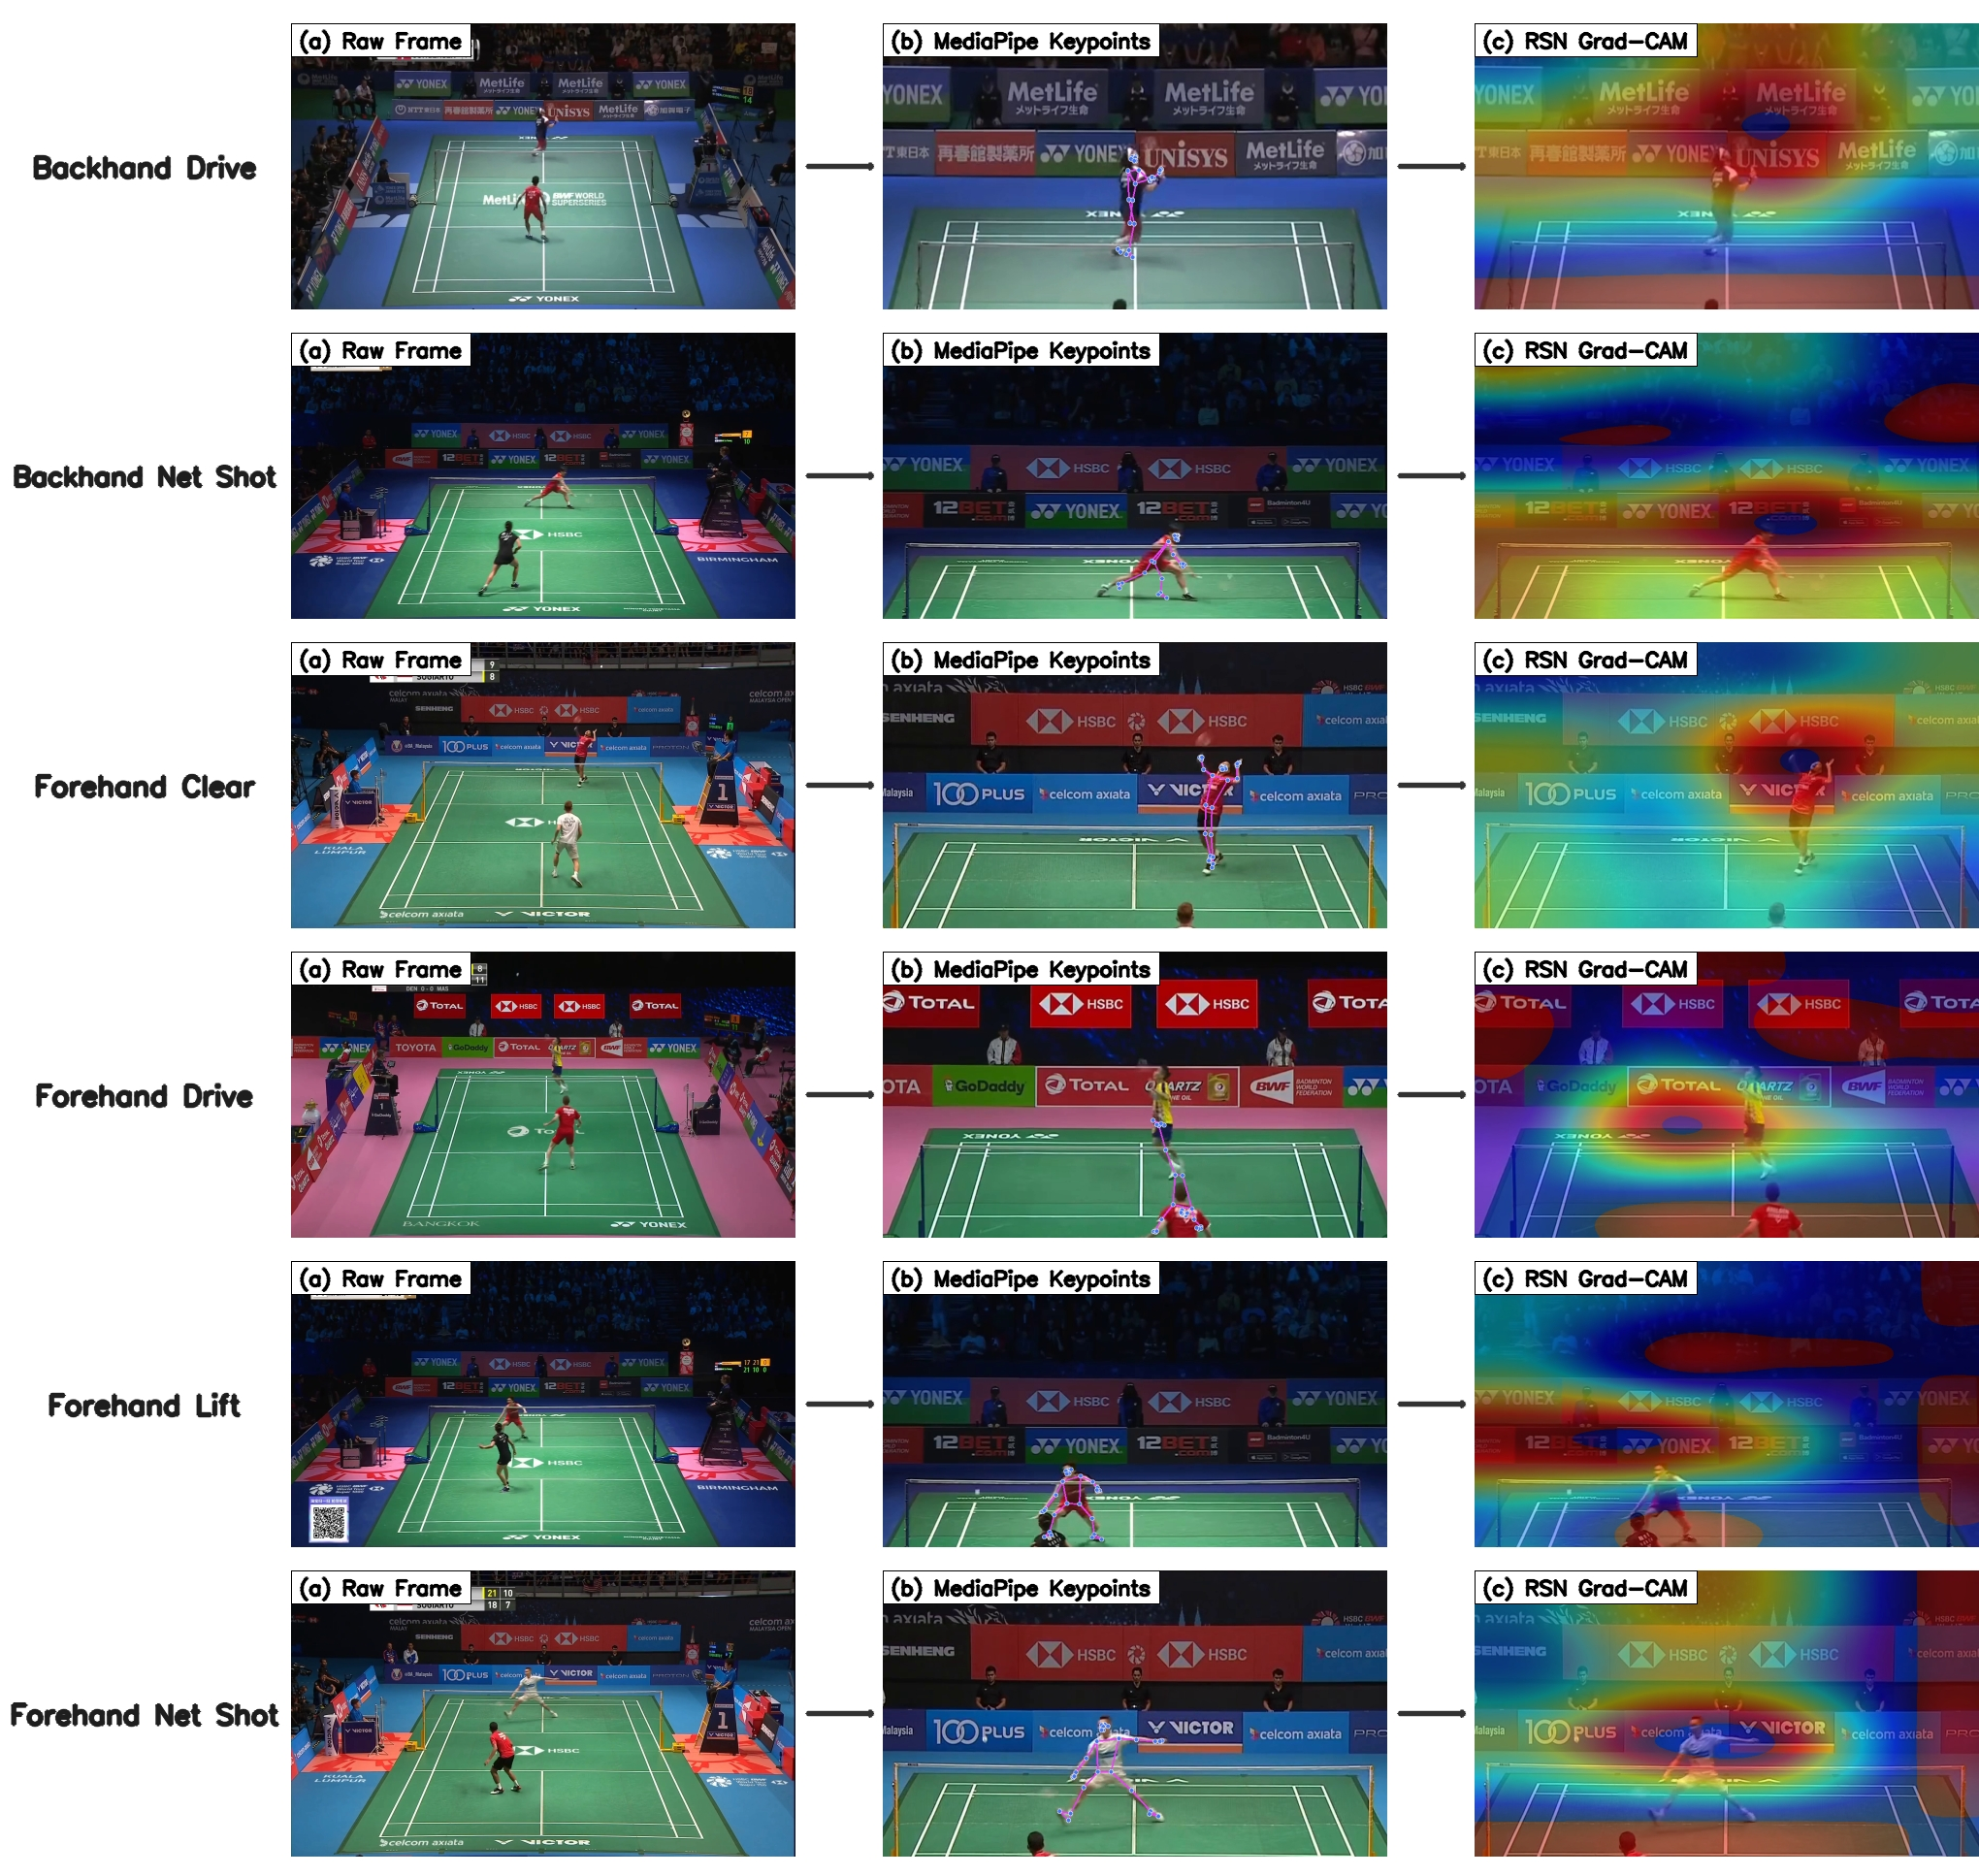
\includegraphics[width=0.98\textwidth]{fig_raw_keypoints_gradcam_per_class.jpg}
\caption{Hybrid feature extraction progression for one exemplar from each of the six shot classes. Each row presents, from left to right: (a) ROI-cropped raw frame, (b) MediaPipe 33-landmark skeletal representation forming the 99-dimensional pose stream, and (c) RSN Grad-CAM activation map forming the 64-dimensional visual stream. The progression highlights how the fused representation captures both kinematic structure and discriminative visual attention before forming the 163-dimensional hybrid vector $x_t$.}\label{fig_feature_pipeline}
\end{figure}

\subsubsection{Geometric Pose Normalization}
The raw 33 three-dimensional landmark coordinates extracted by MediaPipe form a 99-dimensional vector per frame. To ensure the model learns posture geometry rather than camera position or player distance from the camera, a three-step normalization is applied to this landmark matrix $P \in \mathbb{R}^{33\times3}$, visualized in the center column of Fig.~\ref{fig_feature_pipeline}:
\begin{enumerate}
    \item \textbf{Centering:} The skeleton is translated so the hip center $c$ becomes the origin, as defined in Eq.~\eqref{eq:center}:
    \begin{equation}
    c = \frac{P_{LH} + P_{RH}}{2}, \quad \tilde{P} = P - c
    \label{eq:center}
    \end{equation}
    \noindent where $c$ is the midpoint between the Left Hip ($P_{LH}$) and Right Hip ($P_{RH}$), and $\tilde{P}$ represents the translated coordinates.
    
    \item \textbf{Alignment:} A spine vector $s$ is defined from the hip center to the shoulder midpoint. An orthonormal basis $R = [\hat{x}; \hat{y}; \hat{z}]$ is constructed such that the spine aligns with the vertical Y-axis. The pose is rotated via $P' = \tilde{P}R^T$.
    
    \item \textbf{Scaling:} The pose is normalized by the spine length $l = \|s\|$ to achieve scale invariance, as given in Eq.~\eqref{eq:scale}:
    \begin{equation}
    \overline{P} = \frac{P'}{l}
    \label{eq:scale}
    \end{equation}
    \noindent where $\overline{P}$ is the final normalized pose vector and $l$ is the Euclidean length of the user's spine in the frame.
\end{enumerate}
\clearpage
\subsection{Hybrid Feature Engineering}

\subsubsection{Residual-Shuffle Network (RSN) Backbone}
For the Hybrid pipeline, a compact visual embedding is extracted to capture context (e.g., racket position, grip nuances). Unlike conventional approaches that use pre-trained ImageNet models such as MobileNetV2, the Smashifix system employs a custom Residual-Shuffle Network (RSN) inspired by the ShuffleNet V2 \cite{b24} design principles. The RSN is a lightweight, efficient backbone that combines residual connections with channel shuffling for effective cross-group information mixing.

The RSN architecture consists of:
\begin{itemize}
    \item \textbf{Stem:} A $3 \times 3$ convolution with stride 2 followed by batch normalization, ReLU activation, and max pooling for initial feature extraction and spatial downsampling.
    \item \textbf{Shuffle Units (4 Stages):} Each stage comprises multiple Shuffle Units. For stride-1 units, the input channels are split in half: one half passes through an identity shortcut while the other is processed by a bottleneck consisting of $1 \times 1$ Conv $\rightarrow$ Depthwise $3 \times 3$ Conv $\rightarrow$ $1 \times 1$ Conv, each followed by batch normalization and ReLU. For stride-2 units, both branches downsample, effectively doubling the channel count. After concatenation, a channel shuffle operation redistributes information across groups.
    \item \textbf{Global Average Pooling + Projection:} The backbone output is reduced to a global feature vector, projected to $d$ dimensions via a dense layer with ReLU activation, and L2-normalized.
\end{itemize}

The channel shuffle operation is described as a reshape-transpose-flatten sequence on the channel dimension, as expressed in Eq.~\eqref{eq:shuffle}:
\begin{equation}
\text{Shuffle}(x, g) = \text{Flatten}\left(\text{Transpose}\left(\text{Reshape}(x, [B, H, W, g, C/g]), [0,1,2,4,3]\right)\right)
\label{eq:shuffle}
\end{equation}
\noindent where $g$ is the number of groups (set to 4) and $C$ is the total channel count.

The complete stage-wise configuration of the RSN backbone is presented in Table~\ref{tab_rsn_config}. Channels double and spatial resolution halves at each stage, yielding a compact 512-dimensional global descriptor after Global Average Pooling.

\begin{table}[h]
\caption{RSN (Residual-Shuffle Network) Stage Configuration. Each downsampling Shuffle Unit uses stride~2; subsequent units use stride~1. Channels double at each stage boundary.}\label{tab_rsn_config}
\centering
\setlength{\tabcolsep}{5pt}
\renewcommand{\arraystretch}{1.3}
\begin{tabular}{|l|c|c|c|}
\hline
\textbf{Stage} & \textbf{Output Size} & \textbf{Shuffle Units} & \textbf{Channels} \\
\hline
Stem (Conv $3{\times}3$, s2 + BN + ReLU + MaxPool s2) & $56 \times 56$ & -- & 64 \\
\hline
Stage~1 & $28 \times 28$ & 2 & 64 \\
\hline
Stage~2 & $14 \times 14$ & 3 & 128 \\
\hline
Stage~3 & $7 \times 7$ & 3 & 256 \\
\hline
Stage~4 & $4 \times 4$ & 2 & 512 \\
\hline
Global Average Pooling & $1 \times 1$ & -- & 512 \\
\hline
Projection (Dense + ReLU + L2-Norm) & -- & -- & $d{=}64$ \\
\hline
\end{tabular}
\end{table}

\paragraph{Two-Stage RSN Training Procedure.}
The RSN is trained in two phases to produce the compact 64-dimensional visual embedding that constitutes 64 of the 163 dimensions in the hybrid feature vector $x_t$.

\textit{Stage~1 (Supervised Pre-training).}
ROI-cropped frames are extracted offline from training videos and resized to $224 \times 224 \times 3$. Pixel values are rescaled to $[0,1]$. A classification head---Dropout(0.3) $\!\to\!$ Dense(256, ReLU) $\!\to\!$ Dropout(0.3) $\!\to\!$ Dense(6, Softmax)---is appended to the backbone, and the entire network is trained end-to-end for six-class stroke classification. Training uses the Adam optimizer ($\eta = 10^{-3}$), sparse categorical cross-entropy loss, and three callbacks: (i)~model checkpointing saving the best validation-accuracy weights, (ii)~early stopping with patience~10, and (iii)~ReduceLROnPlateau (factor~0.5, patience~3, minimum~$10^{-6}$). The data pipeline leverages cached, shuffled, and prefetched \texttt{tf.data} batches for GPU throughput.

\textit{Stage~2 (Frozen Feature Extraction).}
After convergence, the classification head is discarded and the backbone weights are frozen ($\theta_{\text{RSN}} \leftarrow \text{const}$). A lightweight projection head Dense($d{=}64$, ReLU) followed by L2-normalization replaces the classifier. For each incoming frame $I_t$, the frozen extractor produces a 64-dimensional unit-norm vector $c_t$ capturing racket orientation, grip angle, and shuttle-contact vicinity without overfitting to training identities. This design mirrors transfer-learning practice while remaining computationally inexpensive ($\sim$0.4~GFLOPs per frame). The two-stage procedure is critical: Stage~1 forces the backbone to learn stroke-discriminative visual features, while Stage~2 produces a compact, generalizable embedding suitable for downstream temporal fusion.

The ROI-cropped frame $I_t$ is resized to $224 \times 224$ and passed through the pre-trained RSN to produce the visual feature vector, as given in Eq.~\eqref{eq:rsn}:
\begin{equation}
h_{t} = \text{RSN}(I_{t}) \in \mathbb{R}^{d}
\label{eq:rsn}
\end{equation}
\noindent where $h_t$ is the feature map extracted from input image $I_t$. To interpret which spatial regions drive RSN decisions, Grad-CAM \cite{b31} is computed from the final convolutional feature tensor $A^{k}$ and a target score $y^{c}$. The importance weight of each channel is computed as in Eq.~\eqref{eq:gradcam_alpha}:
\begin{equation}
\alpha_k^{c} = \frac{1}{Z}\sum_i\sum_j \frac{\partial y^{c}}{\partial A_{ij}^{k}}
\label{eq:gradcam_alpha}
\end{equation}
and the activation map is computed as in Eq.~\eqref{eq:gradcam_map}:
\begin{equation}
L_{\text{Grad-CAM}}^{c} = \text{ReLU}\left(\sum_k \alpha_k^{c} A^{k}\right)
\label{eq:gradcam_map}
\end{equation}
\noindent where $\alpha_k^{c}$ is the importance weight of channel $k$ and $Z$ is the number of spatial locations. The map is then bilinearly upsampled to the input resolution and alpha-blended with the ROI frame for visualization. In the rightmost column of Fig.~\ref{fig_feature_pipeline}, high-intensity regions consistently concentrate around the racket head, wrist-elbow chain, and shuttle contact vicinity, indicating that the visual stream captures stroke-discriminative biomechanics.

This embedding is projected to 64 dimensions and L2-normalized, as expressed in Eq.~\eqref{eq:proj}:
\begin{equation}
u_{t} = \text{ReLU}(W h_{t} + b), \quad c_{t} = \frac{u_{t}}{\|u_{t}\|_2}
\label{eq:proj}
\end{equation}
\noindent where $W$ and $b$ are learnable weights and biases, and $c_t$ is the normalized context vector.

\subsubsection{Feature Fusion}
The normalized pose vector and the visual embedding are concatenated to form the final hybrid feature vector $x_t$, as defined in Eq.~\eqref{eq:fusion}:
\begin{equation}
x_{t} = [\text{vec}(\overline{P}_{t}) \parallel c_{t}] \in \mathbb{R}^{163}
\label{eq:fusion}
\end{equation}
Fig.~\ref{fig_feature_pipeline} summarizes the complete dual-stream extraction pipeline, from the raw cropped frame through to the pose and visual embeddings.

\subsubsection{Classification Architecture}
The core classification engine is a dual-stream hybrid architecture combining an Attention-enhanced Temporal Convolutional Network with a late fusion strategy:
\begin{itemize}
    \item \textbf{Visual Branch (Attention-TCN):} The visual feature sequence undergoes an initial $1 \times 1$ projection to $F$ filters, followed by a deep TCN consisting of 4 dilated causal Conv1D layers with dilations $d \in \{1, 2, 4, 8\}$. Each TCN layer includes batch normalization, ReLU activation, spatial dropout, and a residual connection. The exponentially increasing dilation yields a receptive field of 31 frames. The output is then processed by a Multi-Head Self-Attention layer ($h$ heads, key dimension $k$) and a layer-normalized GRU block ($G$ units).
    \item \textbf{Pose Branch:} The normalized pose sequence is independently processed by a Conv1D layer ($F$ filters, kernel size 3, causal padding), followed by an identical Multi-Head Self-Attention block and a GRU layer ($G$ units) with batch normalization.
    \item \textbf{Late Fusion:} The sequence summaries of both branches are concatenated to form a 163-dimensional hybrid feature vector. This vector is passed through two dense layers ($F_{\text{fuse}}$ and $F_{\text{fuse}}/2$ units) with dropout and L2 regularization, terminating in a softmax classifier for final stroke prediction.
\end{itemize}

The dilated causal convolution for layer $l$ with dilation rate $d_l$ is expressed in Eq.~\eqref{eq:dilconv}:
\begin{equation}
\text{DilConv}(x_t, d_l) = \sum_{k=0}^{K-1} w_k \cdot x_{t - d_l \cdot k}
\label{eq:dilconv}
\end{equation}
\noindent where $K$ is the kernel size (set to 3), $w_k$ are the learned filter weights, and the causal constraint ensures $t - d_l \cdot k \ge 0$.

The Multi-Head Self-Attention mechanism is formalized in Eq.~\eqref{eq:attention}:
\begin{equation}
\text{Attention}(Q, K, V) = \text{softmax}\left(\frac{QK^T}{\sqrt{d_k}}\right) V
\label{eq:attention}
\end{equation}
\noindent where $Q$, $K$, and $V$ are the query, key, and value projections of the input sequence, and $d_k$ is the key dimension. The multi-head variant concatenates $h$ independent attention heads and projects the result. A residual connection preserves gradient flow, as shown in Eq.~\eqref{eq:layernorm}:
\begin{equation}
y = \text{LayerNorm}(x + \text{MultiHead}(x, x, x))
\label{eq:layernorm}
\end{equation}

The hyperparameters of the Attention-TCN were optimized using Optuna \cite{b41} with a Bayesian search strategy. The tuned values are: $F = 80$ filters, $G = 80$ GRU units, $h = 8$ attention heads, $k = 32$ key dimension, $F_{\text{fuse}} = 80$ fusion units, L2 regularization $\lambda = 7.6 \times 10^{-5}$, dropout rate $p = 0.22$, learning rate $\eta = 5.6 \times 10^{-4}$, and label smoothing $\epsilon = 0.1$.

\subsubsection{Contact-Aware Prediction Algorithm}
To improve accuracy, the specific temporal window containing the stroke contact point is identified. A composite arm velocity $v_t$ is calculated based on the right shoulder, elbow, and wrist. The window with the maximum acceleration magnitude $A$ is selected for the final prediction, as given in Eq.~\eqref{eq:contact}:
\begin{equation}
A = \|\Delta v\|_2, \quad \text{Class} = \arg\max_{c} p(c | X_{\text{peak\_acc}})
\label{eq:contact}
\end{equation}
\noindent where $A$ is the magnitude of acceleration, and $\Delta v$ represents the change in velocity vectors between consecutive frames.

\subsection{Biomechanical Analysis (KSI Algorithm)}



The core of the feedback mechanism is the enhanced Kinematic Similarity Index (KSI), which compares the user's motion sequence $U$ against a DTW-aligned expert template $E$. KSI extends the original algorithm with 32 hierarchical biomechanical features, contact-centered windowing, confidence filtering, and jerk analysis.

The complete KSI computation is formalized in Algorithm~\ref{alg:ksi}.


\subsubsection{Enhanced Feature Extraction (32D)}
KSI extracts 32 hierarchical biomechanical features per frame, organized into six categories:
\begin{itemize}
    \item \textbf{Joint Angles (12):} Elbow flexion, shoulder elevation, shoulder abduction, knee flexion, hip flexion, and ankle dorsiflexion for both left and right sides.
    \item \textbf{Limb Ratios (6):} Full arm extension, full leg extension, and forearm-to-upper-arm ratio, normalized by torso length for scale invariance.
    \item \textbf{Spinal Alignment (4):} Forward lean (sagittal), lateral lean (frontal), spine twist (transverse), and normalized spine length.
    \item \textbf{Rotational Dynamics (4):} Hip-shoulder separation angle (critical for power generation), hip rotation, shoulder rotation, and trunk rotation velocity.
    \item \textbf{Wrist Dynamics (3):} Wrist height, horizontal reach, and radial deviation---all normalized relative to the torso.
    \item \textbf{Center of Mass (3):} Approximate CoM displacement in $x$, $y$, and $z$ axes, computed as a weighted average of hip (50\%), shoulder (30\%), and knee (20\%) positions.
\end{itemize}
\begin{algorithm}[htbp]
\caption{   Kinematic Similarity Index (KSI)}
\label{alg:ksi}
\begin{algorithmic}[1]
\Require User landmarks $\mathbf{U} \in \mathbb{R}^{T_U \times 33 \times 3}$, Expert template $\mathbf{E} \in \mathbb{R}^{T_E \times 33 \times 3}$, Weights $\mathbf{w} = (w_p, w_v, w_a)$, Confidence threshold $\tau$, Band ratio $\beta$
\Ensure KSI score $S \in [0,1]$, Per-joint error map $\mathcal{E}$, Feedback vector $\mathbf{F}$
\Statex
\State \textbf{--- Stage 1: Confidence Filtering ---}
\For{each frame $t$ in $\mathbf{U}$ and $\mathbf{E}$}
    \State Reject if mean landmark visibility $< \tau$
    \State Reject if any limb-length ratio falls outside anthropometric bounds
    \State Reject if $\max_j \|\mathbf{p}_j^{\,t} - \mathbf{p}_j^{\,t-1}\|_2 > 0.3$ \Comment{temporal artifact}
\EndFor
\State $\hat{\mathbf{U}} \leftarrow$ valid user frames; \quad $\hat{\mathbf{E}} \leftarrow$ valid expert frames
\Statex
\State \textbf{--- Stage 2: Shot-Phase Segmentation \& Contact Windowing ---}
\State $v_t \leftarrow \|\Delta\, \hat{\mathbf{E}}_{\text{R\_wrist}}\|$ \Comment{racket-arm wrist velocity}
\State $t_c \leftarrow \arg\max_t\, v_t$ \Comment{contact frame}
\State $\hat{\mathbf{E}} \leftarrow \hat{\mathbf{E}}[\,t_c - W_{\text{pre}} \;:\; t_c + W_{\text{post}}\,]$
\State $\hat{\mathbf{U}} \leftarrow$ similarly windowed user sequence
\State Segment into phases: \textsc{Preparation, Loading, Acceleration, Contact, Follow-Through}
\Statex
\State \textbf{--- Stage 3: Hierarchical Feature Extraction (32-D) ---}
\For{each frame $t$ in $\hat{\mathbf{U}}$ and $\hat{\mathbf{E}}$}
    \State $\mathbf{f}_t \leftarrow \textsc{Extract}_{32}(\text{angles, ratios, spine, rotation, wrist, CoM})$
\EndFor
\State Compute trunk rotation velocity: $\dot{\phi}_t \leftarrow \nabla_t(\text{hip-shoulder separation})$
\Statex
\State \textbf{--- Stage 4: DTW Alignment with Sakoe-Chiba Band ---}
\State $r \leftarrow \lfloor \beta \cdot \max(T_E, T_U) \rfloor$ \Comment{band width}
\State Fill cost matrix $D_{i,j}$ subject to $|i-j| \le r$
\State Backtrack optimal path $\mathcal{W}^{*}$; produce aligned pair $(\tilde{\mathbf{E}},\, \tilde{\mathbf{U}})$
\Statex
\State \textbf{--- Stage 5: Phase-Aware Attention Weights ---}
\For{each aligned frame $k$}
    \State $\alpha_k \leftarrow w_{\text{phase}} \cdot \bigl(0.5 + 0.5\,\exp\!\bigl(-{(k - \mu_{\text{phase}})^2}/{2\sigma_{\text{phase}}^2}\bigr)\bigr)$
\EndFor
\Statex
\State \textbf{--- Stage 6: Multi-Component Scoring ---} 
\State $S_{\text{pose}} \leftarrow {\sum_k \alpha_k \cos(\tilde{\mathbf{E}}_k, \tilde{\mathbf{U}}_k)}/{\sum_k \alpha_k}$
\State $S_{\text{vel}} \leftarrow {\sum_k \alpha_k \cdot \cos_{\text{vel},k} \cdot \exp(-0.1\|V_k^E - V_k^U\|^2)}/{\sum_k \alpha_k}$
\State $S_{\text{acc}} \leftarrow$ analogous formulation on second derivatives
\State $S \leftarrow w_p \cdot S_{\text{pose}} + w_v \cdot S_{\text{vel}} + w_a \cdot S_{\text{acc}}$
\Statex
\State \textbf{--- Stage 7: Per-Joint Error Analysis \& Feedback ---}
\For{each feature $i \in \{1, \dots, 32\}$}
    \State $\mathcal{E}_i \leftarrow (\bar{e}_i,\; e_i^{\max},\; \sigma_i,\; t_i^{\text{crit}},\; \text{CI}_{95\%})$ via adaptive bootstrap
    \If{$\bar{e}_i > \theta_{\text{severity}}$}
        \State Append biomechanical correction to $\mathbf{F}$ via causal-chain lookup
    \EndIf
\EndFor
\State \Return $S,\; \mathcal{E},\; \mathbf{F}$
\end{algorithmic}
\end{algorithm}++++         

\subsubsection{Confidence Filtering}
Before analysis, unreliable frames are filtered based on two criteria:
\begin{enumerate}
    \item \textbf{Anatomical Plausibility:} Limb length ratios are checked against expected anthropometric ranges. Frames with anatomically implausible configurations are rejected.
    \item \textbf{Temporal Consistency:} Frames exhibiting sudden landmark displacements exceeding 0.3 (in normalized coordinates) between consecutive frames are flagged as tracking artifacts and excluded.
\end{enumerate}

\subsubsection{Contact-Centered Windowing}
To focus computational resources on the most biomechanically relevant portion of the sequence, a contact-centered window is applied. The contact frame $t_c$ is identified from the shot phase segmentation, and a window of $\pm W$ frames is extracted around it, as defined in Eq.~\eqref{eq:window}:
\begin{equation}
\text{Window} = [t_c - W_{\text{pre}}, \; t_c + W_{\text{post}}]
\label{eq:window}
\end{equation}
\noindent where $W_{\text{pre}}$ and $W_{\text{post}}$ are the pre-contact and post-contact window sizes (set to 18 frames each, covering approximately 600ms at 30 FPS).

\subsubsection{Dynamic Time Warping (DTW) with Sakoe-Chiba Band}
To account for temporal variations in execution speed, DTW aligns the sequences by minimizing the cumulative Euclidean distance. The recurrence relation for the cost matrix $D$ is given in Eq.~\eqref{eq:dtw}:
\begin{equation}
D_{i,j} = \|F_{i}^{E} - F_{j}^{U}\|_2 + \min\{D_{i-1,j}, D_{i,j-1}, D_{i-1,j-1}\}
\label{eq:dtw}
\end{equation}
\noindent where:
\begin{itemize}
    \item $D_{i,j}$: The cumulative cost to align Expert frame $i$ with User frame $j$.
    \item $F_{i}^{E}, F_{j}^{U}$: The biomechanical feature vectors for the Expert and User respectively.
    \item $\|\cdot\|_2$: The Euclidean distance metric.
\end{itemize}

To improve computational efficiency and prevent pathological alignments, a Sakoe-Chiba band constraint \cite{b42} is applied, restricting the warping path to a band of width $r$ around the diagonal, as expressed in Eq.~\eqref{eq:sacoe}:
\begin{equation}
|i - j| \le r, \quad r = \lfloor \beta \cdot \max(N_E, N_U) \rfloor
\label{eq:sacoe}
\end{equation}
\noindent where $\beta$ is the band ratio (set to 0.2) and $N_E$, $N_U$ are the lengths of the expert and user sequences respectively.

\subsubsection{Phase-Aware Attention}
The system segments the aligned shot into five biomechanical phases: \textit{Preparation, Loading, Acceleration, Contact,} and \textit{Follow-through}. An attention weight $\alpha_k$ is assigned to each frame using a Gaussian envelope centered on the phase, as expressed in Eq.~\eqref{eq:attn_weight}:
\begin{equation}
\alpha_{k} = w_{\text{phase}} \cdot \left(0.5 + 0.5\exp\left(-0.5\left(\frac{k-\text{center}}{\text{width}}\right)^{2}\right)\right)
\label{eq:attn_weight}
\end{equation}
\noindent where:
\begin{itemize}
    \item $\alpha_k$: The importance weight assigned to frame $k$.
    \item $w_{\text{phase}}$: The predefined weight of the current phase, with Contact phase $w=3.0$, Acceleration phase $w=2.0$, and Preparation phase $w=0.8$.
    \item $\text{center}$: The frame index representing the midpoint of the phase.
    \item $\text{width}$: A parameter controlling the spread of the Gaussian curve.
\end{itemize}

\subsubsection{Scoring Components}
The final KSI score is an aggregate of four differential kinematic similarities.

\textbf{Pose Similarity ($S_{\text{pose}}$):} Computed as the attention-weighted cosine similarity of the feature vectors, as given in Eq.~\eqref{eq:spose}:
\begin{equation}
S_{\text{pose}} = \frac{\sum_{k}\alpha_{k} \cdot \frac{F_k^E \cdot F_k^U}{\|F_k^E\| \cdot \|F_k^U\|}}{\sum_{k}\alpha_{k}}
\label{eq:spose}
\end{equation}

\textbf{Velocity Similarity ($S_{\text{vel}}$):} Incorporates both directional alignment and magnitude matching, as defined in Eq.~\eqref{eq:svel}:
\begin{equation}
S_{\text{vel}} = \frac{\sum_{k}\alpha_{k} \cdot \text{cos}_{\text{vel},k} \cdot \exp(-0.1\|V_k^E - V_k^U\|^2)}{\sum_{k}\alpha_{k}}
\label{eq:svel}
\end{equation}
\noindent where $\text{cos}_{\text{vel},k}$ is the cosine similarity between the User's and Expert's velocity directions at frame $k$, and $V^E$, $V^U$ are the respective velocity magnitudes.

\textbf{Acceleration Similarity ($S_{\text{acc}}$)} and \textbf{Jerk Similarity ($S_{\text{jerk}}$)} follow analogous formulations using the second and third temporal derivatives of the feature sequences, respectively.

The final weighted KSI score is computed as given in Eq.~\eqref{eq:ksi_total}:
\begin{equation}
\text{KSI}_{\text{total}} = w_p \cdot S_{\text{pose}} + w_v \cdot S_{\text{vel}} + w_a \cdot S_{\text{acc}}
\label{eq:ksi_total}
\end{equation}
\noindent where $w_p = 0.4$, $w_v = 0.4$, and $w_a = 0.2$ are the component weights.
As illustrated in Fig.~\ref{fig2}, the detailed model architecture and end-to-end prediction pipeline show the flow from video input through pose estimation, feature extraction, dual-pipeline classification, and KSI-based biomechanical feedback generation.


\subsubsection{Natural Language Coaching Generation}
While the KSI provides a rigorous mathematical foundation for identifying errors, numerical indices alone lack the actionable context required by amateur players. To bridge this gap, Smashifix integrates a Natural Language Coach that transforms raw KSI outputs into personalized, pedagogically structured coaching reports. The module is composed of three principal components: a Biomechanical Knowledge Base, a multi-stage feedback generation pipeline, and a skill-adaptive language engine.

\paragraph{Biomechanical Knowledge Base.}
The foundation of the coach is an expert-authored knowledge base encoding domain-specific biomechanical causality chains. For each of the 32 features monitored by the KSI (Algorithm~\ref{alg:ksi}), the knowledge base stores: (i)~a set of observable \textit{symptoms} (e.g., ``elbow too straight'', ``arm dropping''), (ii)~a causal chain mapping each symptom to underlying biomechanical causes---for instance, the racket arm elbow dropping may stem from rotator cuff fatigue, habitual bad form, or an excessively tight grip---(iii)~the governing biomechanical principle explaining the kinetic chain role of that joint (e.g., ``the elbow acts as a velocity multiplier; optimal angle 90--$120^{\circ}$ allows maximum angular velocity transfer from shoulder to wrist''), and (iv)~shot-specific priority rankings indicating which features are most critical for each of the six stroke types.

\paragraph{Error Classification and Causal Reasoning.}
The KSI per-joint error map $\mathcal{E}$ is first classified into four severity tiers using configurable thresholds on the effective error magnitude:
\begin{itemize}
    \item \textbf{Critical} ($\geq 25^{\circ}$): Fundamental biomechanical fault requiring immediate correction.
    \item \textbf{Major} ($\geq 15^{\circ}$): Significant deviation impacting power or consistency.
    \item \textbf{Minor} ($\geq 8^{\circ}$): Detectable deviation with marginal performance impact.
    \item \textbf{Negligible} ($< 8^{\circ}$): Within acceptable biomechanical tolerance.
\end{itemize}
Shot-specific priority features receive a $1.5\times$ severity boost (top two priorities) or $1.2\times$ (secondary priorities), so that wrist contact height and hip-shoulder separation are weighted more heavily for a Forehand Clear than for a Net Shot. For the top three errors (two Critical, one Major), the coach traverses the causal chain to determine the most likely root cause and selects the corresponding correction strategy.

\paragraph{Skill-Level Adaptive Language.}
The system supports four skill levels---Beginner, Intermediate, Advanced, and Expert---and dynamically adjusts its vocabulary, explanatory depth, and prescribed drills accordingly. Table~\ref{tab_skill_adapt} illustrates this adaptation for correcting insufficient hip-shoulder separation:

\begin{table}[h]
\caption{Skill-Level Adaptation: Hip-Shoulder Separation Correction}\label{tab_skill_adapt}
\centering
\small
\setlength{\tabcolsep}{4pt}
\renewcommand{\arraystretch}{1.3}
\begin{tabular}{|l|p{10.5cm}|}
\hline
\textbf{Level} & \textbf{Generated Correction} \\
\hline
Beginner & ``Turn your body like you're throwing a ball sideways. Hips face forward first, then shoulders catch up.'' \\
\hline
Intermediate & ``Create `X-factor' stretch: rotate hips $30^{\circ}$ toward target while shoulders stay back, then unwind explosively.'' \\
\hline
Advanced & ``Target 15--$25^{\circ}$ separation at peak. Initiate with hip rotation from ground force; let shoulders lag 40--60\,ms.'' \\
\hline
Expert & ``Optimize stretch-shortening cycle timing. Peak separation should occur 80--100\,ms before contact.'' \\
\hline
\end{tabular}
\end{table}

Each correction is accompanied by a structured coaching item containing: (i)~the issue and severity rating, (ii)~the root-cause explanation from the causal chain, (iii)~a skill-appropriate fix, (iv)~a specific drill with equipment requirements and duration, (v)~a visual mental cue (e.g., ``picture wringing a wet towel''), (vi)~common mistakes to avoid, and (vii)~observable success indicators. Beyond individual corrections, the coach generates phase-by-phase analysis (Preparation through Follow-Through), timing feedback based on peak-velocity offset relative to the expert template, power feedback derived from velocity ratios, a progressive four-week training plan, and a motivational closing message.

\paragraph{Example System Output.}
Table~\ref{tab_coach_example} presents an abridged coaching report generated by Smashifix for a real user performing a Backhand Net Shot at the Intermediate skill level, with a KSI score of $S = 0.35$.

\begin{table}[h]
\caption{Abridged Coaching Report (Backhand Net Shot, KSI\,=\,0.35, Intermediate)}\label{tab_coach_example}
\centering
\small
\setlength{\tabcolsep}{4pt}
\renewcommand{\arraystretch}{1.2}
\begin{tabular}{|l|p{10.5cm}|}
\hline
\textbf{Field} & \textbf{Generated Content} \\
\hline
Rating & $\bigstar$ Foundation Building \\
\hline
Summary & ``Let's rebuild your Backhand Net Shot from the ground up. Your score of 0.35 indicates fundamental technique issues, but small changes will create big improvements!'' \\
\hline
Priority Fix & \textbf{Trunk Posture} ($151.8^{\circ}$ deviation, Critical): ``Maintain 5--$10^{\circ}$ forward lean at contact. Core engaged (like bracing for a punch). Excessive lean = weak shots.'' Drill: Broomstick overhead shadow footwork, 5\,min/session. \\
\hline
Timing & ``Early peak: reaching maximum speed 533\,ms too early. Delay your forward swing initiation.'' \\
\hline
Power & ``Excellent power generation! Matching expert racket head speed.'' \\
\hline
Strengths & Arm extension positioning ($<5^{\circ}$ error); acceleration phase score 0.85. \\
\hline
\end{tabular}
\end{table}

This structured output demonstrates how the system converts a single numerical KSI score into a rich, multi-dimensional coaching narrative that addresses \textit{what} is wrong, \textit{why} it occurs, and \textit{how} to fix it---with progressive specificity adapted to the player's current ability. The full report additionally includes a four-week training plan with week-by-week drill progressions, video timestamp annotations for key error frames, and---for Advanced/Expert users---a technical appendix listing raw component scores ($S_{\text{pose}}$, $S_{\text{vel}}$, $S_{\text{acc}}$, $S_{\text{jerk}}$), DTW distance, and 95\% bootstrap confidence intervals.



\section{Experiments and Results}\label{sec5}

\subsection{Dataset Description}
The system was trained on the Badminton Stroke Video Dataset sourced from Kaggle \cite{b43}, augmented with proprietary high-definition footage. The dataset comprises 1.32 GB of data capturing human subjects performing strokes from multiple angles under consistent lighting conditions. It is categorized into six distinct stroke classes: Forehand Clear, Forehand Drive, Forehand Lift, Forehand Net Shot, Backhand Drive, and Backhand Net Shot. The data was partitioned using a stratified split into a Training Set of 70\%, a Validation Set of 15\%, and a Test Set of 15\%.

Representative frames from each stroke class are shown in Fig.~\ref{fig_dataset_samples}.

\begin{figure}[htbp]
\centering
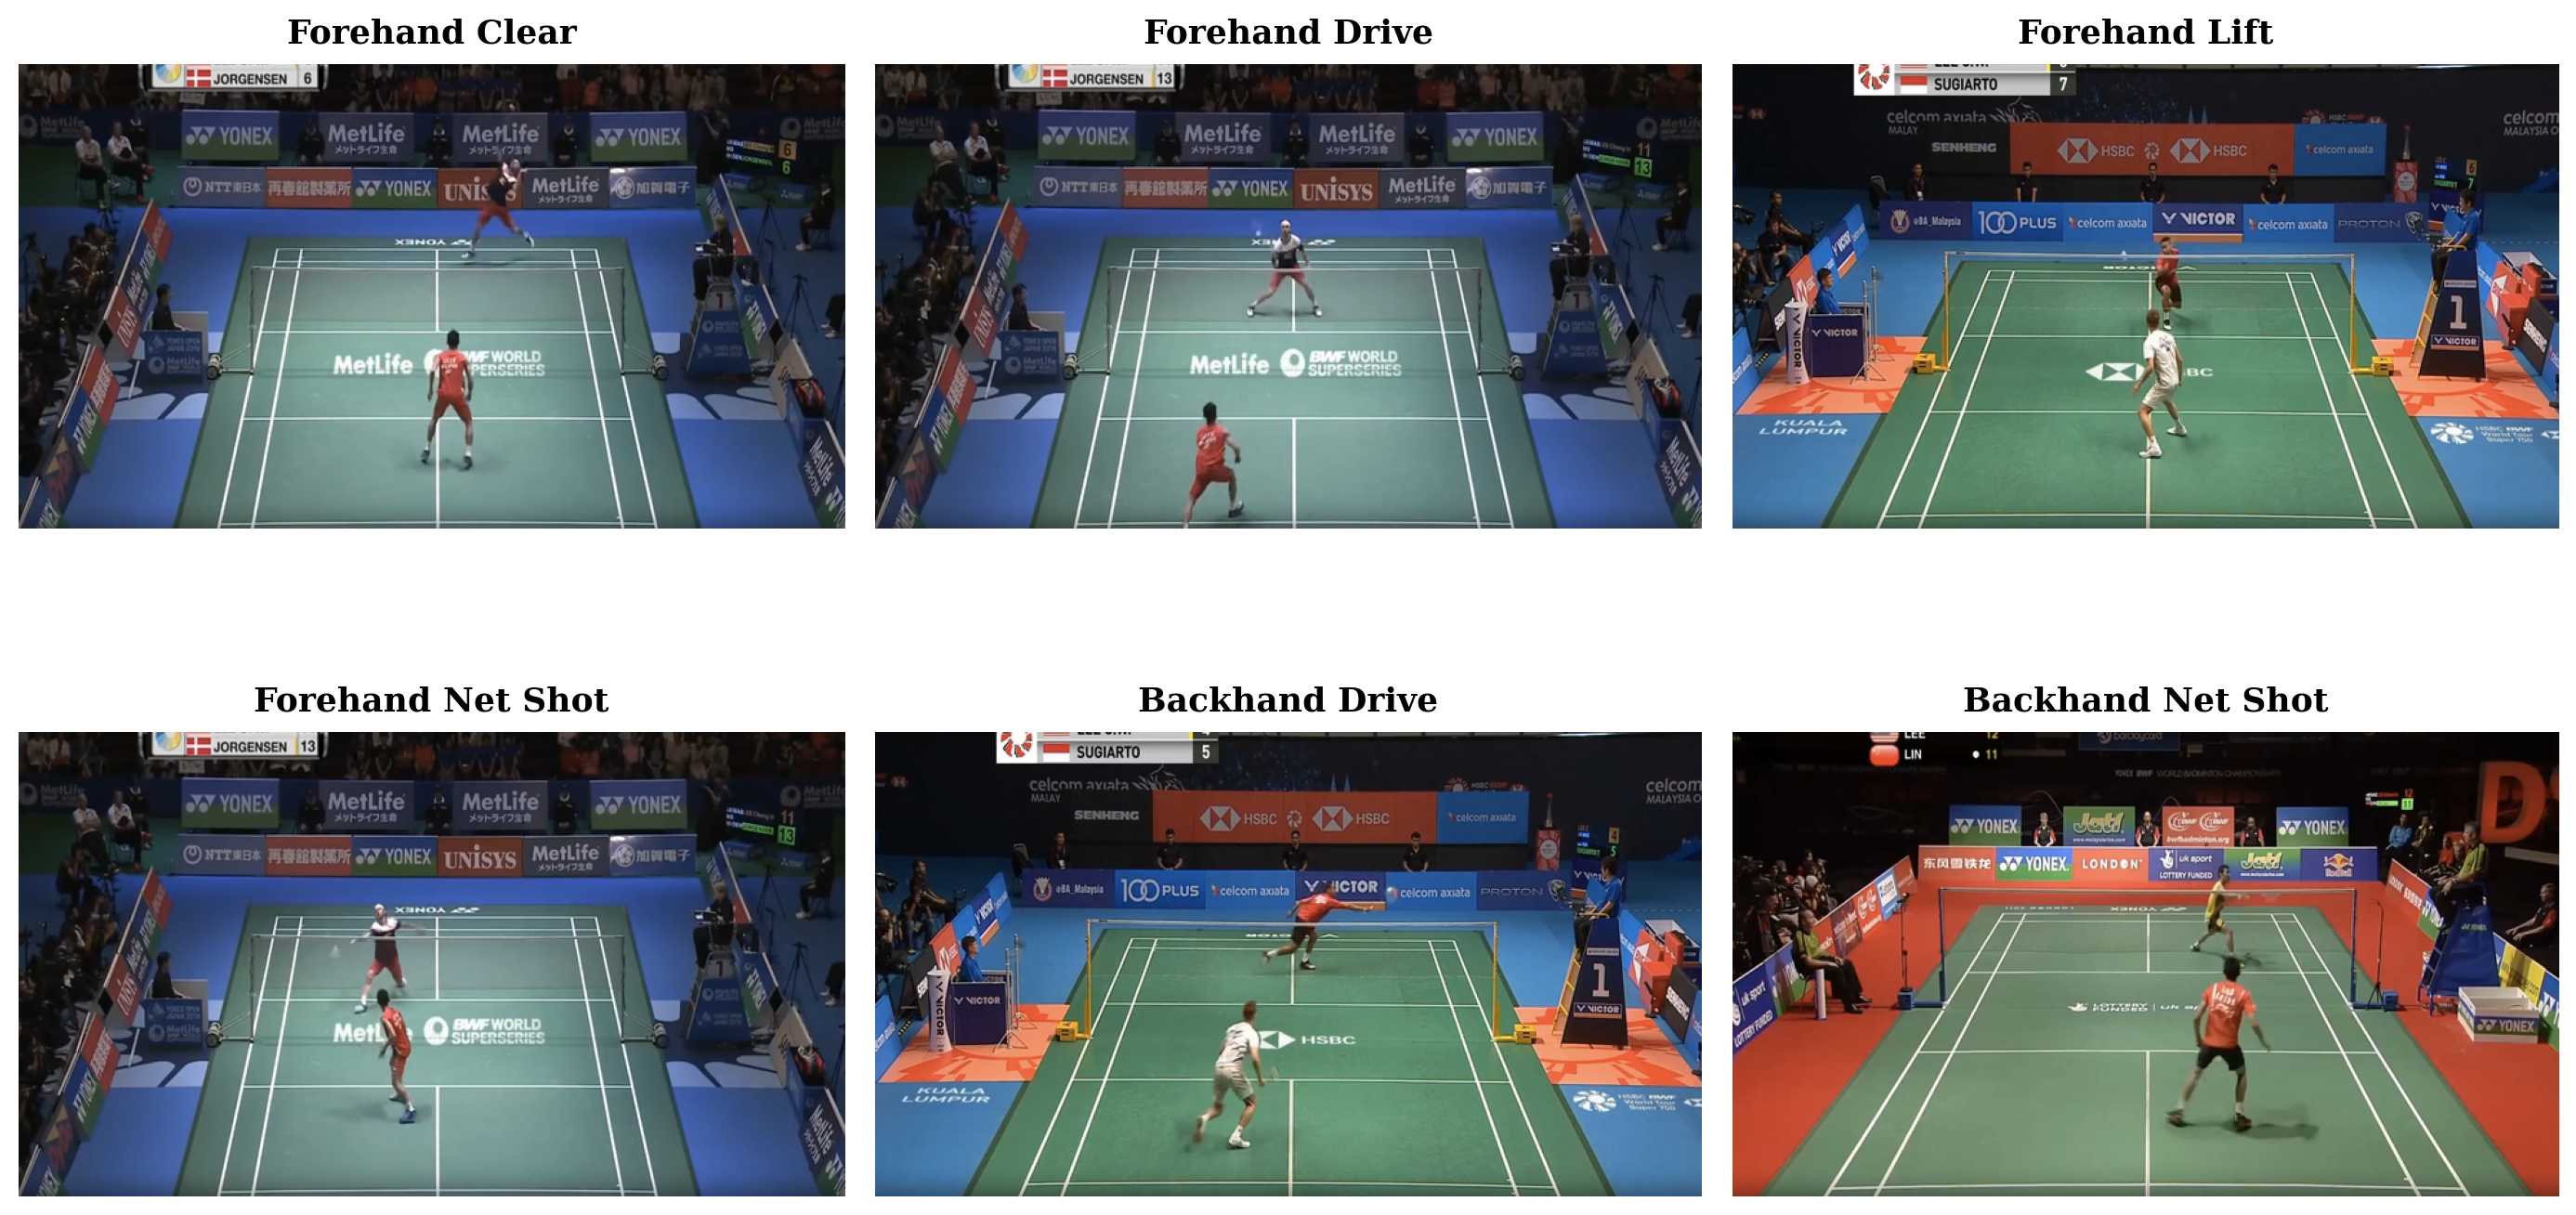
\includegraphics[width=0.95\textwidth]{fig_dataset_samples.png}
\caption{Dataset Sample Frames: one representative frame from each of the six badminton stroke classes, captured from monocular video under consistent lighting conditions.}\label{fig_dataset_samples}
\end{figure}

Fig.~\ref{fig_class_dist} presents the distribution of samples across all six stroke classes for the training, validation, and test splits, demonstrating the balanced representation achieved through stratified sampling.

\begin{figure}[htbp]
\centering
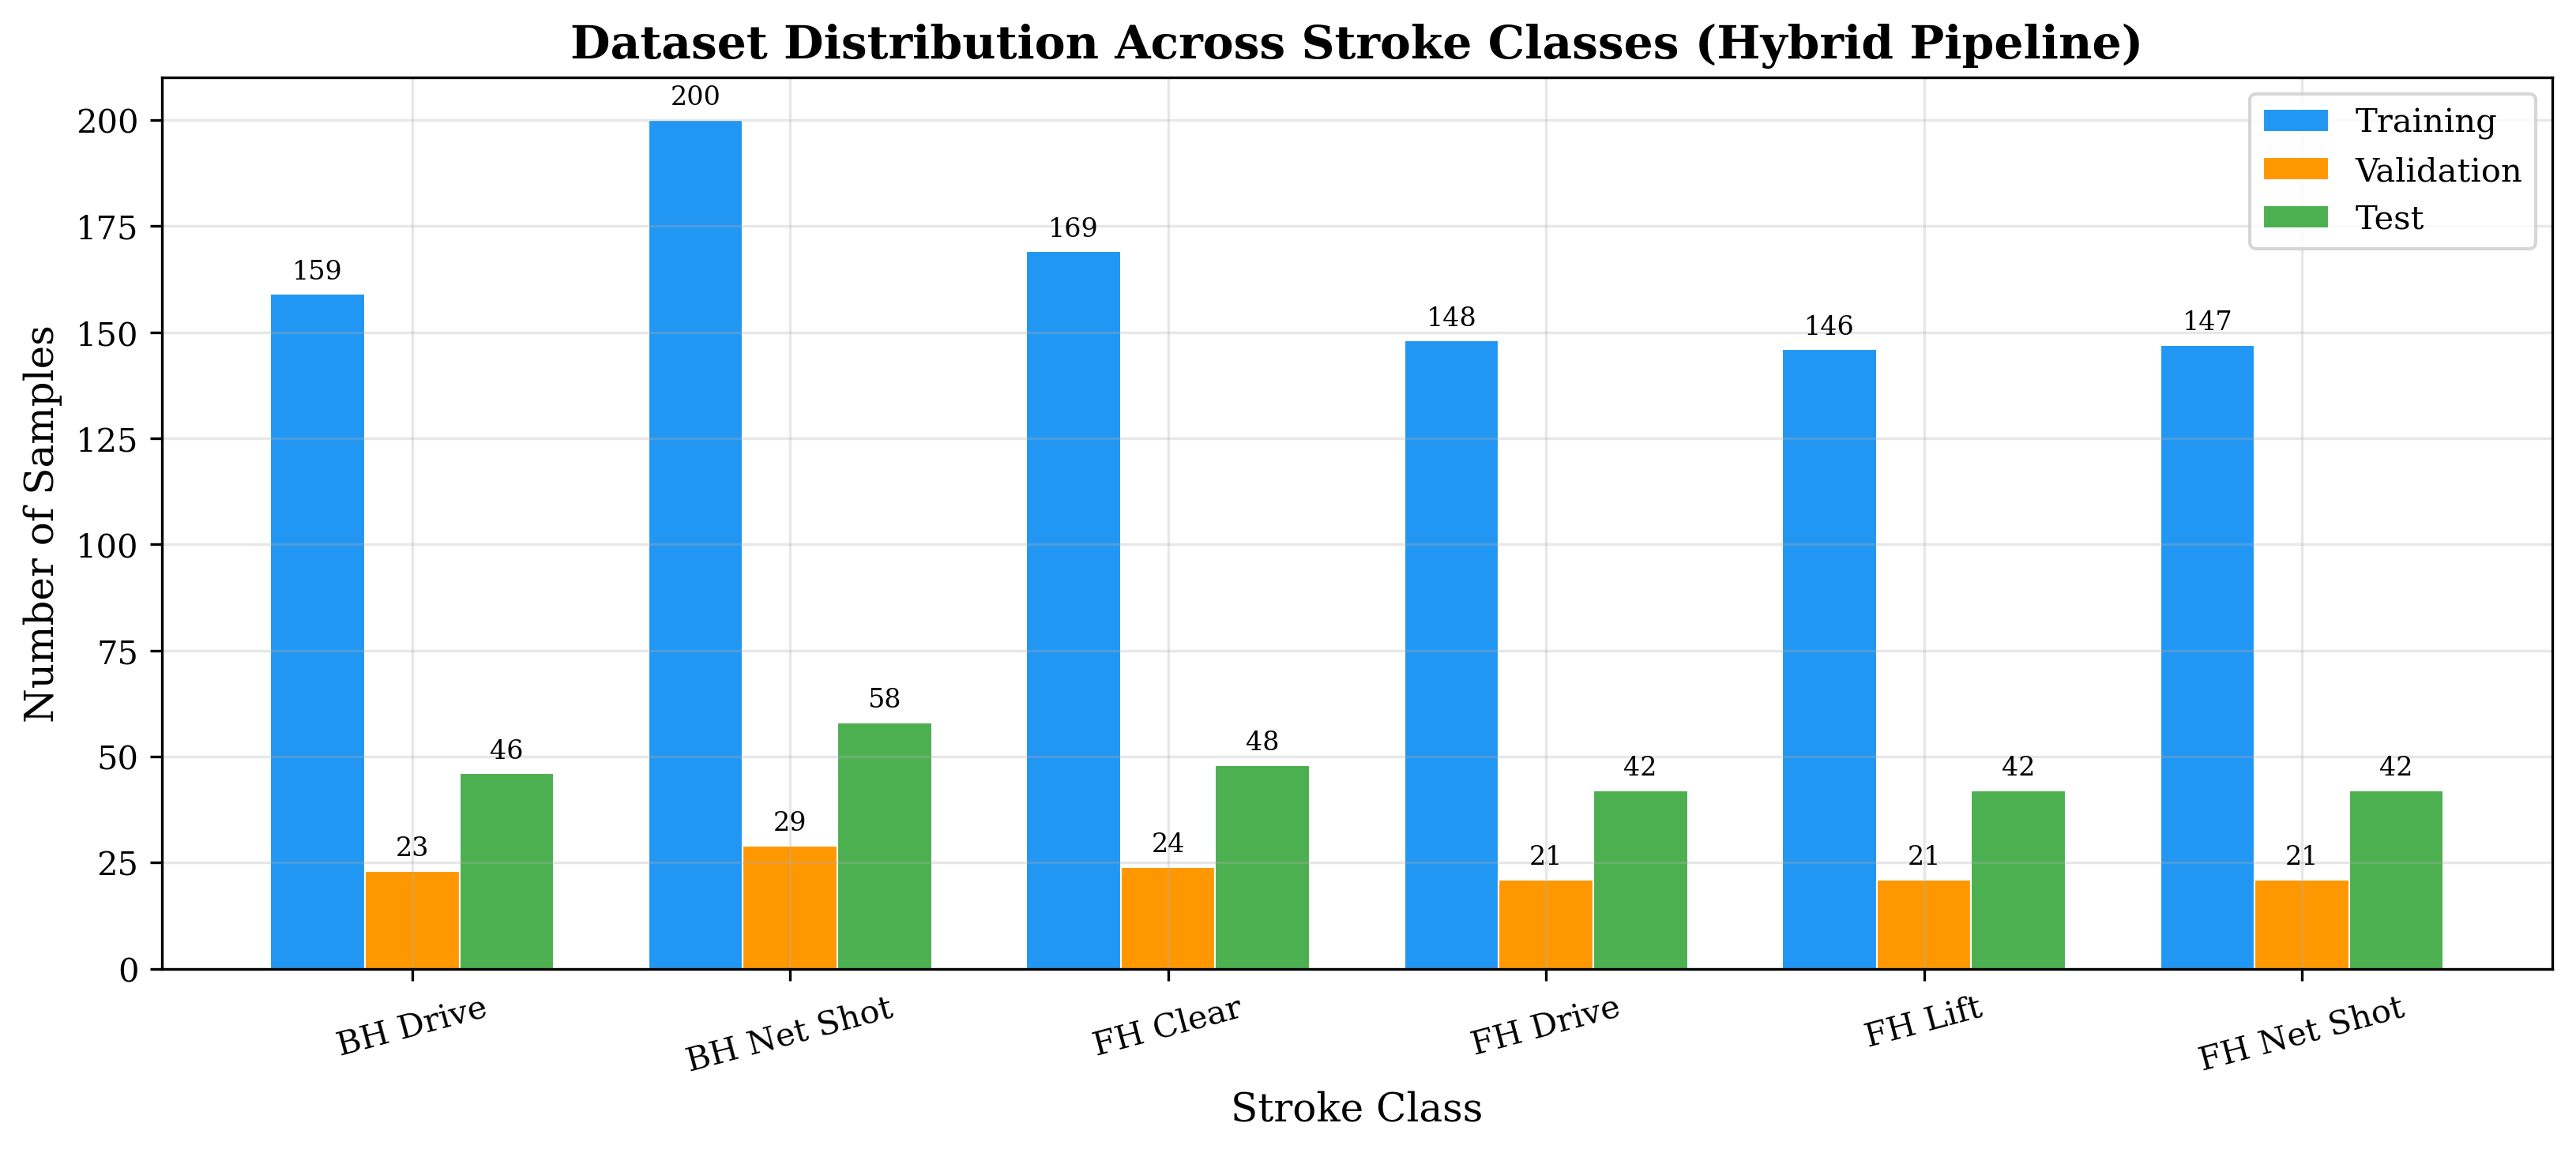
\includegraphics[width=0.85\textwidth]{fig_class_distribution.png}
\caption{Class Distribution Across Splits}\label{fig_class_dist}
\end{figure}

Fig.~\ref{fig2} depicts the end-to-end prediction pipeline of the Smashifix system, showing the complete flow from video input through preprocessing, dual-stream feature extraction, classification, and KSI-driven feedback generation.

\begin{figure}[htbp]
\centering
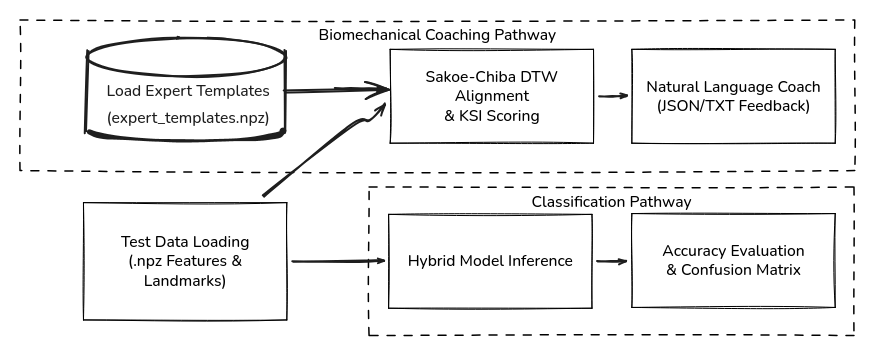
\includegraphics[width=0.98\textwidth]{IPD system Prediction architecture.png}
\caption{End-to-End Prediction Pipeline: the complete flow from raw video input through spatial cropping, pose estimation, RSN visual feature extraction, dual-stream Attention-TCN classification, and KSI-based Natural Language feedback generation.}\label{fig2}
\end{figure}

\subsection{Evaluation Metrics}
To rigorously assess the performance of the classification pipelines, the following metrics were employed:

\begin{enumerate}
    \item \textbf{Accuracy:} The ratio of correctly predicted observations to the total observations, as defined in Eq.~\eqref{eq:accuracy}:
    \begin{equation}
        \text{Accuracy} = \frac{TP + TN}{TP + TN + FP + FN}
        \label{eq:accuracy}
    \end{equation}
    
    \item \textbf{Precision:} The ratio of correctly predicted positive observations to the total predicted positives, as given in Eq.~\eqref{eq:precision}:
    \begin{equation}
        \text{Precision} = \frac{TP}{TP + FP}
        \label{eq:precision}
    \end{equation}
    
    \item \textbf{Recall:} The ratio of correctly predicted positive observations to all observations in the actual class, as given in Eq.~\eqref{eq:recall}:
    \begin{equation}
        \text{Recall} = \frac{TP}{TP + FN}
        \label{eq:recall}
    \end{equation}
    
    \item \textbf{F1-Score:} The weighted average of Precision and Recall, as computed in Eq.~\eqref{eq:f1}:
    \begin{equation}
        F1 = 2 \cdot \frac{\text{Precision} \cdot \text{Recall}}{\text{Precision} + \text{Recall}}
        \label{eq:f1}
    \end{equation}
\end{enumerate}
\noindent where $TP$ = True Positives, $TN$ = True Negatives, $FP$ = False Positives, and $FN$ = False Negatives.

\subsection{Quantitative Results}
The performance of the proposed pipelines on the held-out test set (20\% stratified split, $n=278$) is summarized in Table \ref{tab_results}. The Attention-TCN pipeline demonstrated superior performance due to the inclusion of visual context features and temporal self-attention, achieving a test accuracy of 98.56\% and a macro-averaged F1-Score of 0.98, significantly outperforming both the pose-only and visual-only baselines.

\begin{table}[h]
\caption{Classification Performance Results}\label{tab_results}
\centering
\setlength{\tabcolsep}{6pt}
\renewcommand{\arraystretch}{1.3}
\begin{tabular}{|l|c|c|c|c|}
\hline
\textbf{Model Architecture} & \textbf{Accuracy} & \textbf{Precision} & \textbf{Recall} & \textbf{F1-Score} \\
\hline
Pose-LSTM (Real-time) & 0.81 & 0.79 & 0.78 & 0.78 \\
\hline
\textbf{Attention-TCN (Proposed)} & \textbf{0.9856} & \textbf{0.99} & \textbf{0.98} & \textbf{0.98} \\
\hline
RSN (Visual only) & 0.74 & 0.72 & 0.71 & 0.71 \\
\hline
\end{tabular}
\end{table}

To provide granular insight into the model's discriminative capability across individual stroke types, Table \ref{tab_perclass} presents the per-class precision, recall, and F1-score on the same test set. All six classes achieve F1-scores $\ge 0.98$, with Forehand Clear attaining perfect scores. The slight reduction in recall for Forehand Drive (0.95) indicates occasional confusion with visually similar strokes such as Forehand Lift, which remains a known challenge in badminton action recognition.

\begin{table}[h]
\caption{Attention-TCN Per-Class Classification Metrics}\label{tab_perclass}
\centering
\setlength{\tabcolsep}{5pt}
\renewcommand{\arraystretch}{1.3}
\begin{tabular}{|l|c|c|c|c|}
\hline
\textbf{Shot Class} & \textbf{Precision} & \textbf{Recall} & \textbf{F1-Score} & \textbf{Support} \\
\hline
Backhand Drive & 0.96 & 1.00 & 0.98 & 46 \\
\hline
Backhand Net Shot & 0.98 & 1.00 & 0.99 & 58 \\
\hline
Forehand Clear & 1.00 & 1.00 & 1.00 & 48 \\
\hline
Forehand Drive & 1.00 & 0.95 & 0.98 & 42 \\
\hline
Forehand Lift & 1.00 & 0.98 & 0.99 & 42 \\
\hline
Forehand Net Shot & 0.98 & 0.98 & 0.98 & 42 \\
\hline
\textbf{Macro Average} & \textbf{0.99} & \textbf{0.98} & \textbf{0.98} & \textbf{278} \\
\hline
\end{tabular}
\end{table}

\subsection{Training Dynamics}
The training dynamics of both pipelines are illustrated through their epoch-wise accuracy and loss curves. Fig.~\ref{fig_tcn_curves} shows the Attention-TCN training over 193 epochs, reaching a peak validation accuracy of 94.70\% at epoch 165. The model exhibits slight overfitting in later epochs, with training accuracy exceeding validation accuracy, though the gap remains modest. Fig.~\ref{fig_lstm_curves} depicts the Pose-LSTM training over 71 epochs, converging to a best validation accuracy of 90.44\% at epoch 59, demonstrating faster but lower-ceiling convergence compared to the TCN.

Fig.~\ref{fig_tcn_curves} illustrates the training and validation curves for the Attention-TCN pipeline over 193 epochs: (a) accuracy progression showing peak validation accuracy of 94.70\% at epoch 165, and (b) corresponding loss curves demonstrating consistent convergence.

\begin{figure}[htbp]
\centering
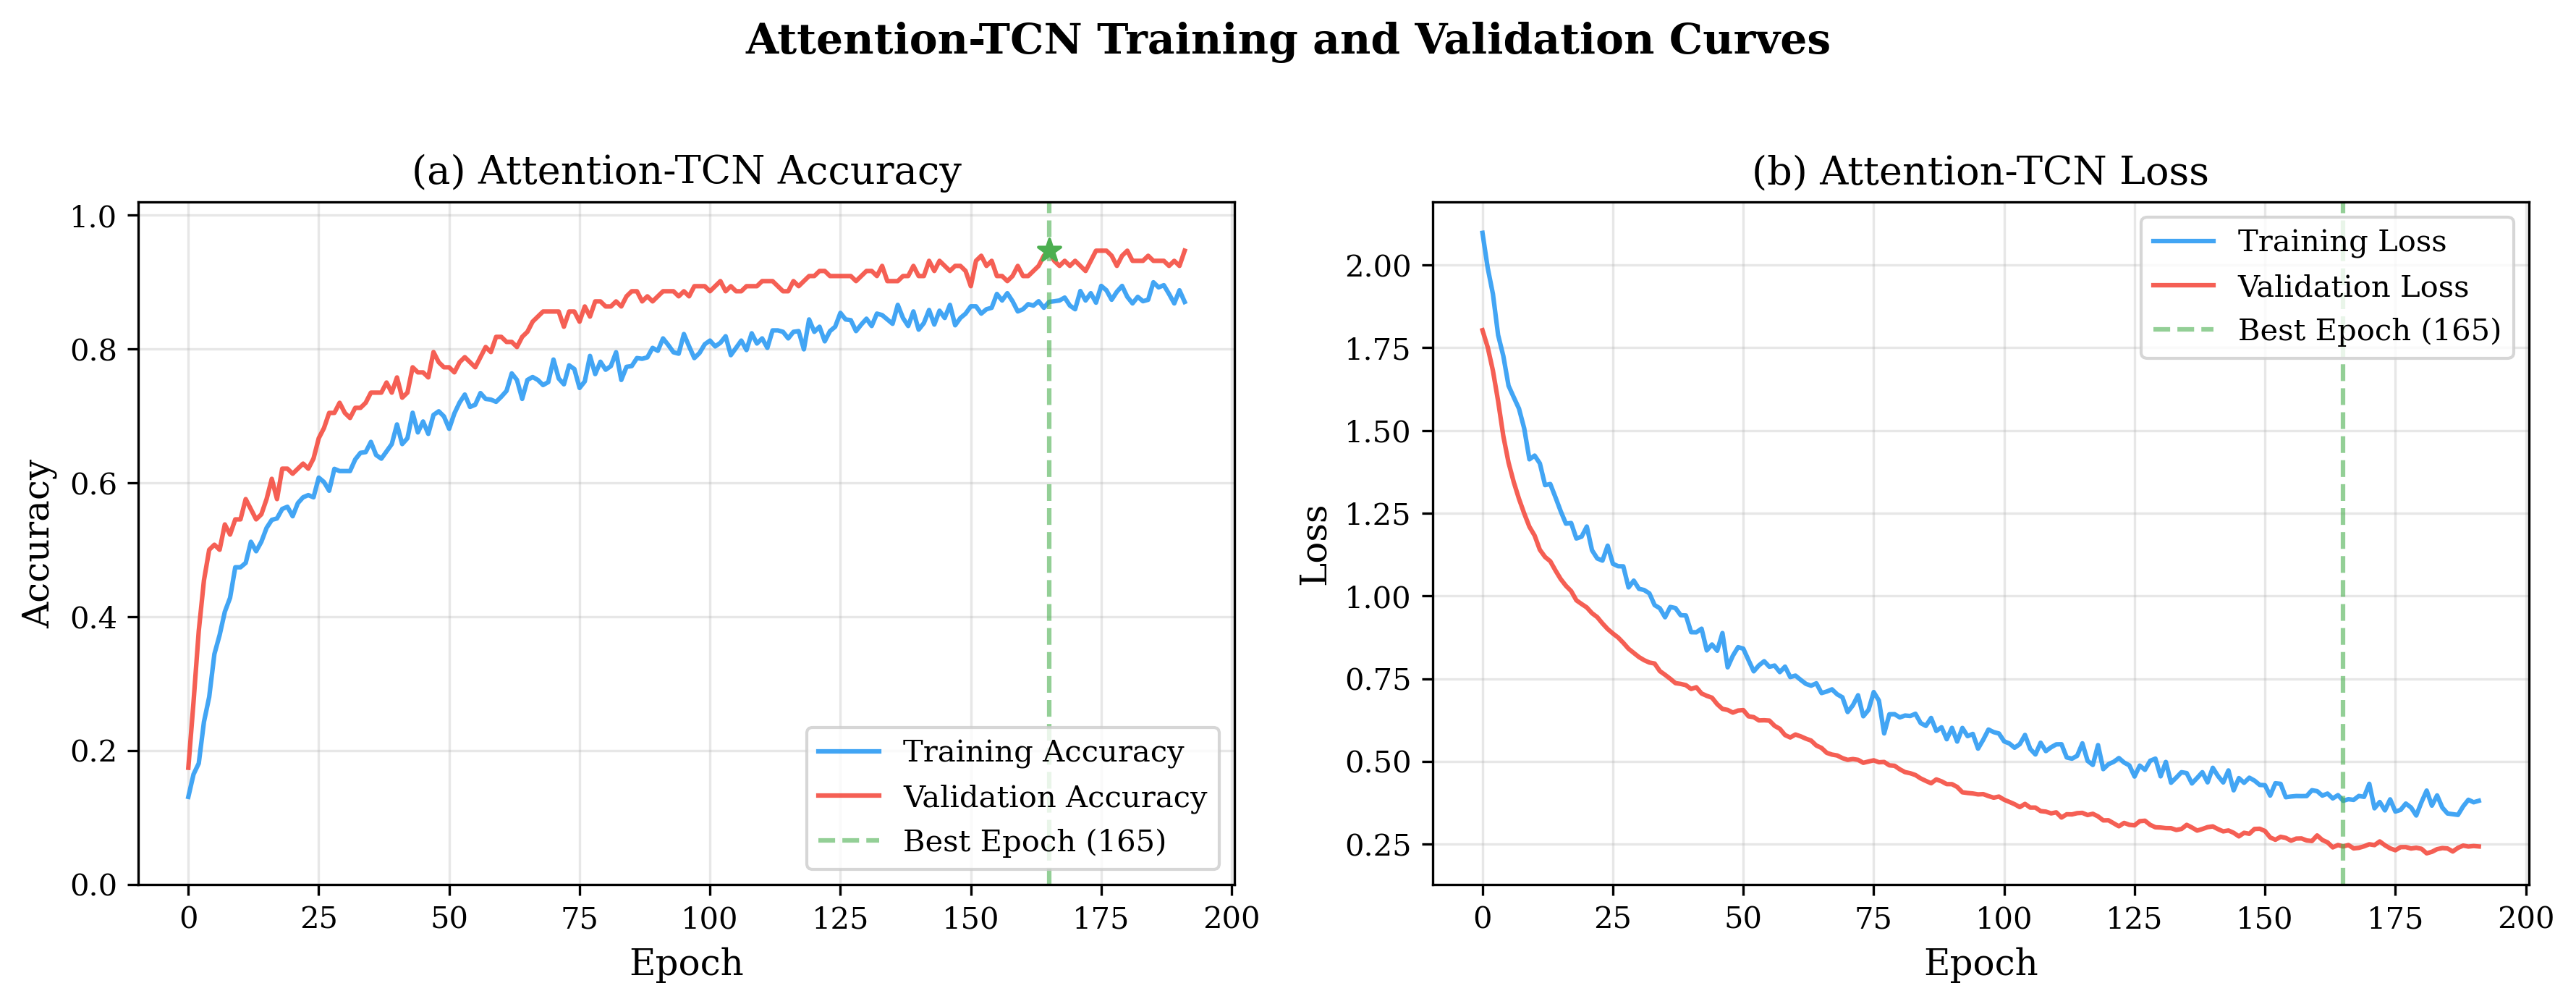
\includegraphics[width=0.95\textwidth]{fig_tcn_training_curves.png}
\caption{Attention-TCN Training Curves}\label{fig_tcn_curves}
\end{figure}

Fig.~\ref{fig_lstm_curves} presents the training and validation curves for the Pose-LSTM pipeline over 71 epochs: (a) accuracy progression showing peak validation accuracy of 90.44\% at epoch 59, and (b) corresponding loss curves with characteristic LSTM oscillation during convergence.

\begin{figure}[htbp]
\centering
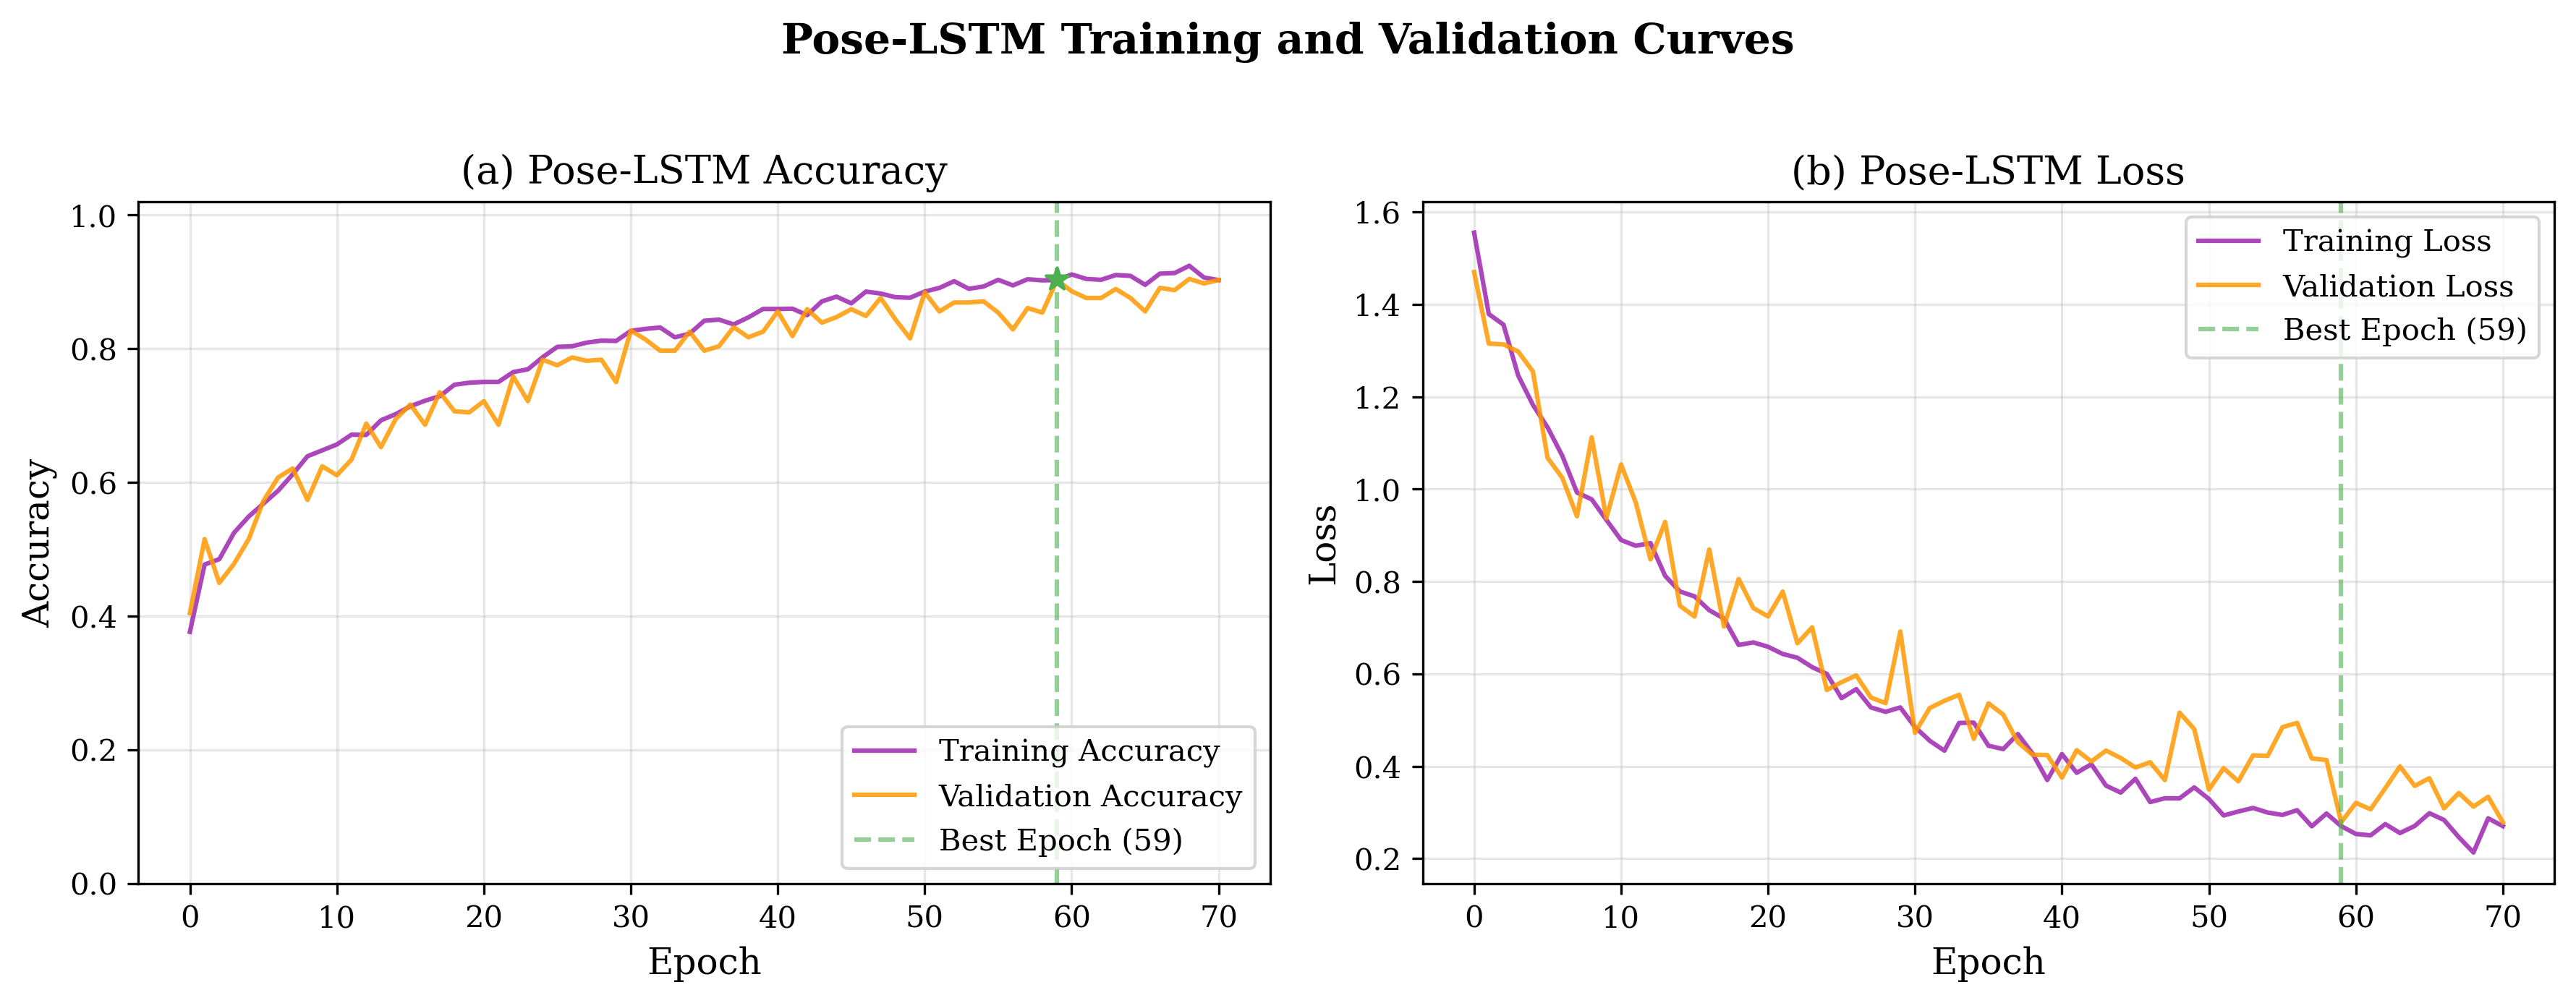
\includegraphics[width=0.95\textwidth]{fig_lstm_training_curves.png}
\caption{Pose-LSTM Training Curves}\label{fig_lstm_curves}
\end{figure}

A direct comparison of the validation accuracy trajectories of both models is presented in Fig.~\ref{fig_model_compare}. The overlay reveals that while the Pose-LSTM initially learns faster due to its simpler architecture and lower-dimensional input, the Attention-TCN ultimately surpasses it after approximately 60 epochs, benefiting from the richer visual context and temporal attention mechanism.

As depicted in Fig.~\ref{fig_model_compare}, an overlay comparison of validation accuracy between the Attention-TCN and Pose-LSTM pipelines illustrates the TCN's superior long-term convergence despite the LSTM's faster initial learning rate.

\begin{figure}[htbp]
\centering
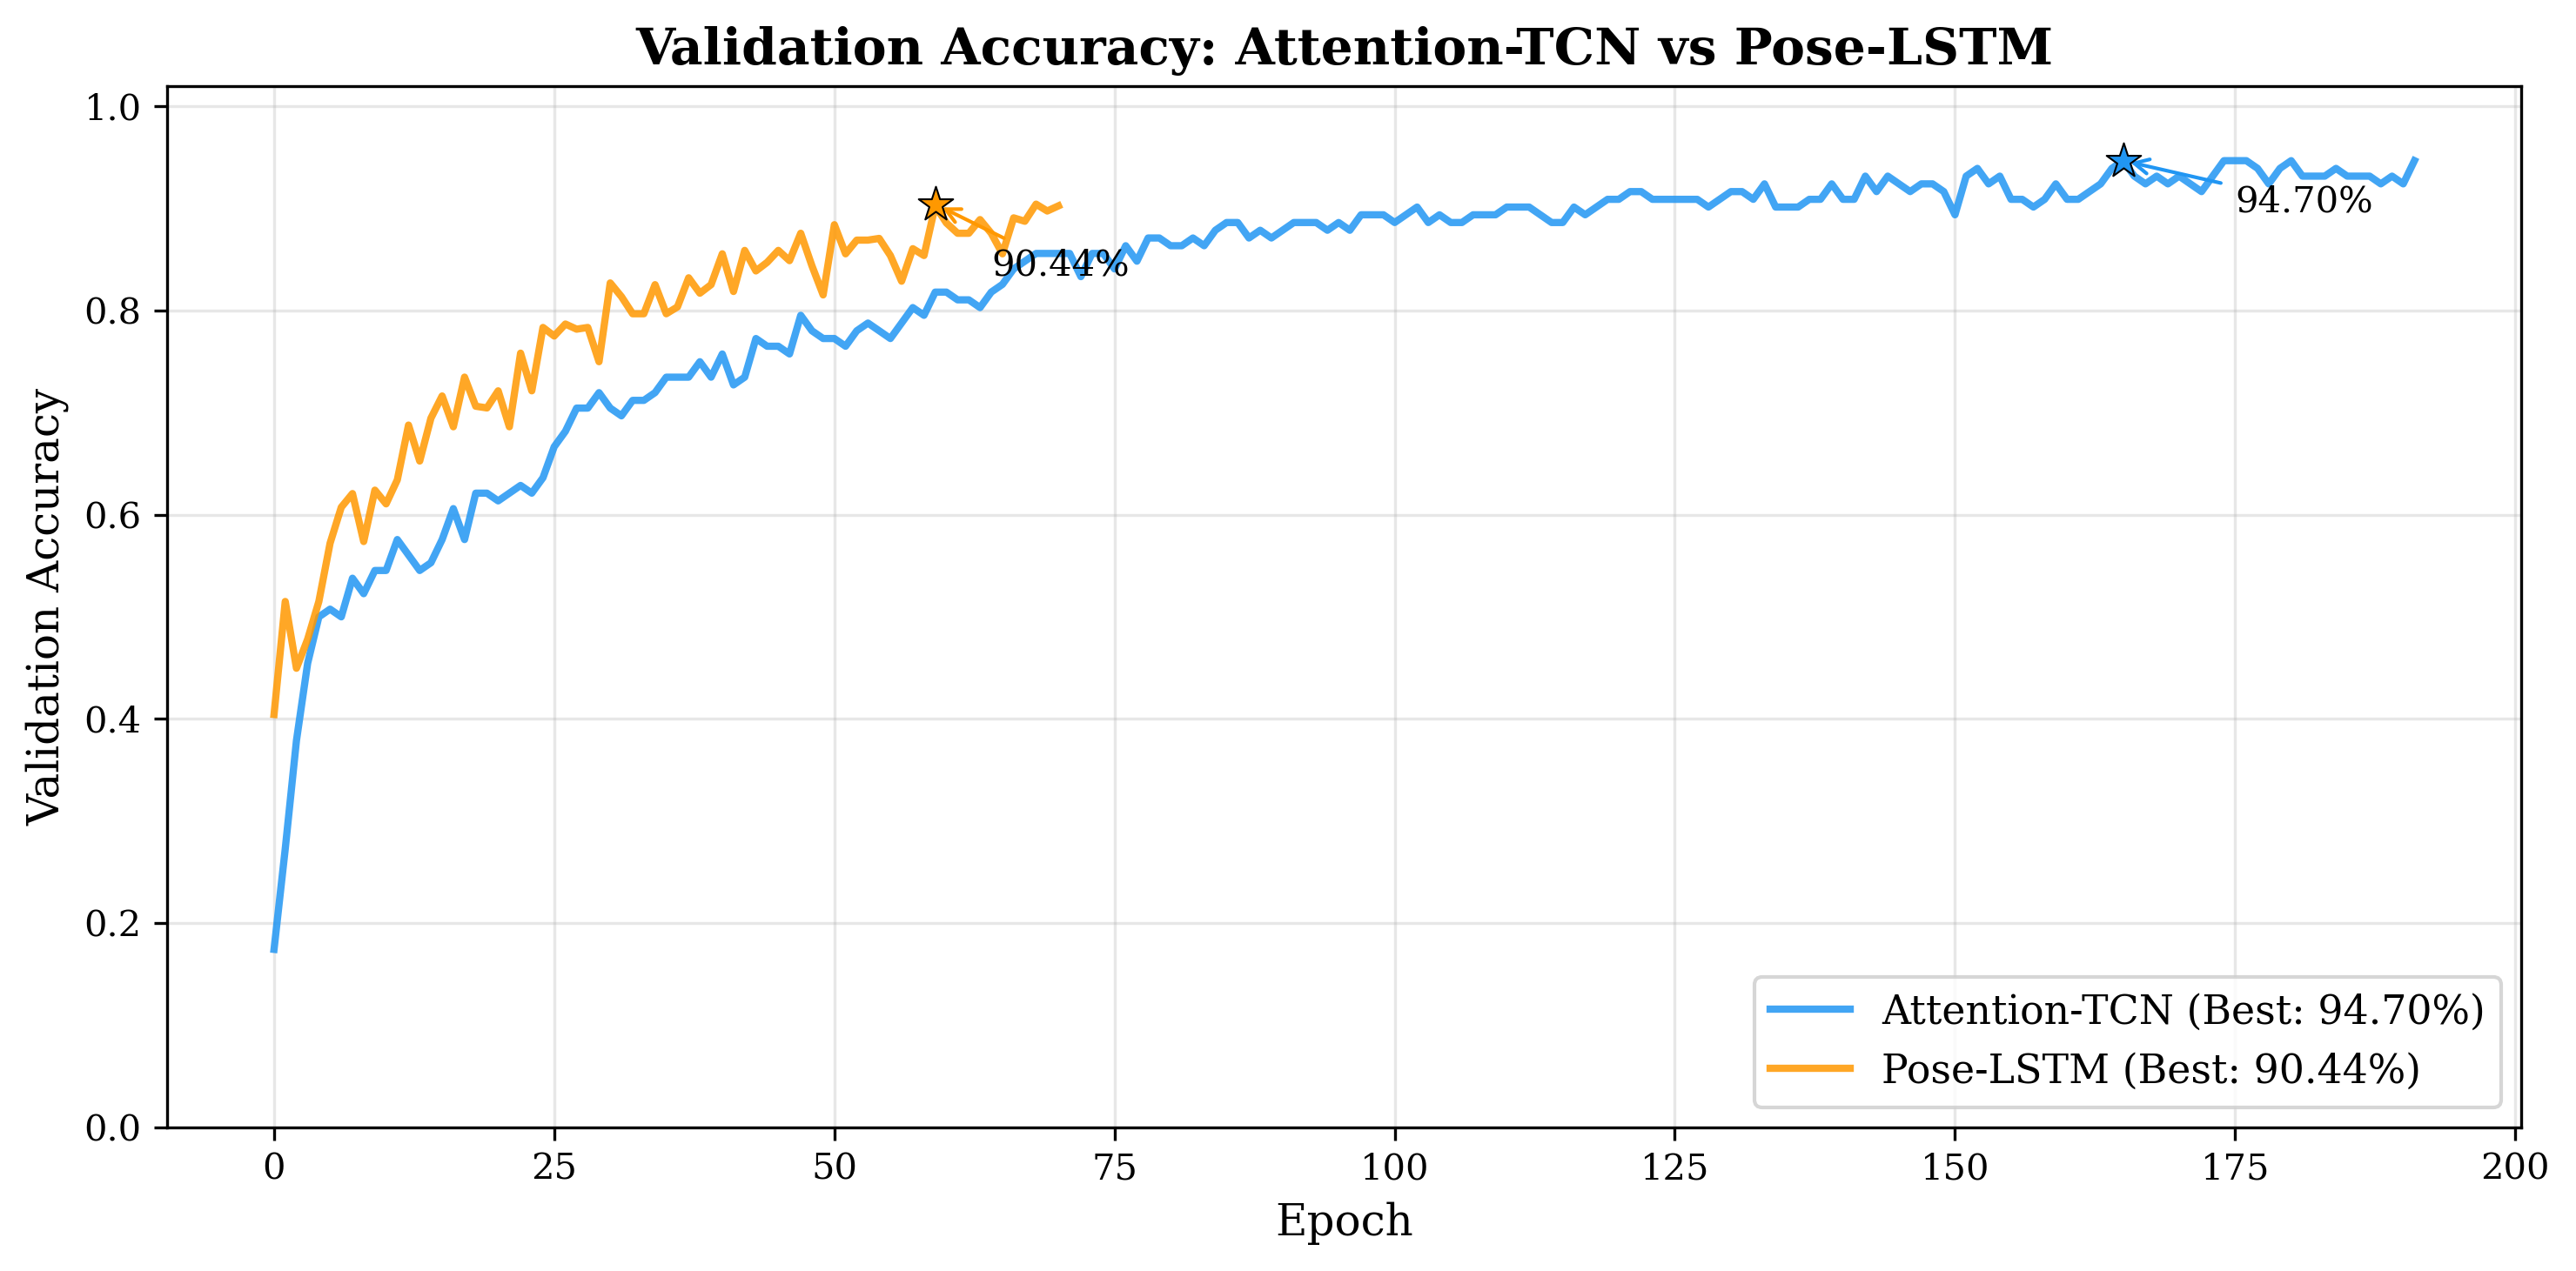
\includegraphics[width=0.85\textwidth]{fig_model_comparison.png}
\caption{Validation Accuracy Overlay Comparison}\label{fig_model_compare}
\end{figure}

\subsection{Hyperparameter Optimization}
The Attention-TCN architecture was optimized using Optuna with Bayesian Tree-structured Parzen Estimator (TPE) sampling over 46 trials. The search space included learning rate, number of TCN filters, attention heads, key dimension, GRU units, dropout rates, and batch size. Fig.~\ref{fig_optuna} presents the validation accuracy achieved by each trial, with a running-best line showing the optimization trajectory. The best configuration achieved 98.92\% validation accuracy at trial 13, after which the marginal returns from additional trials diminished.

Fig.~\ref{fig_optuna} shows the Optuna hyperparameter optimization results for the Attention-TCN over 46 trials using TPE sampling, with bars colour-coded by validation accuracy and a running-best line showing convergence to 98.92\%.

\begin{figure}[htbp]
\centering
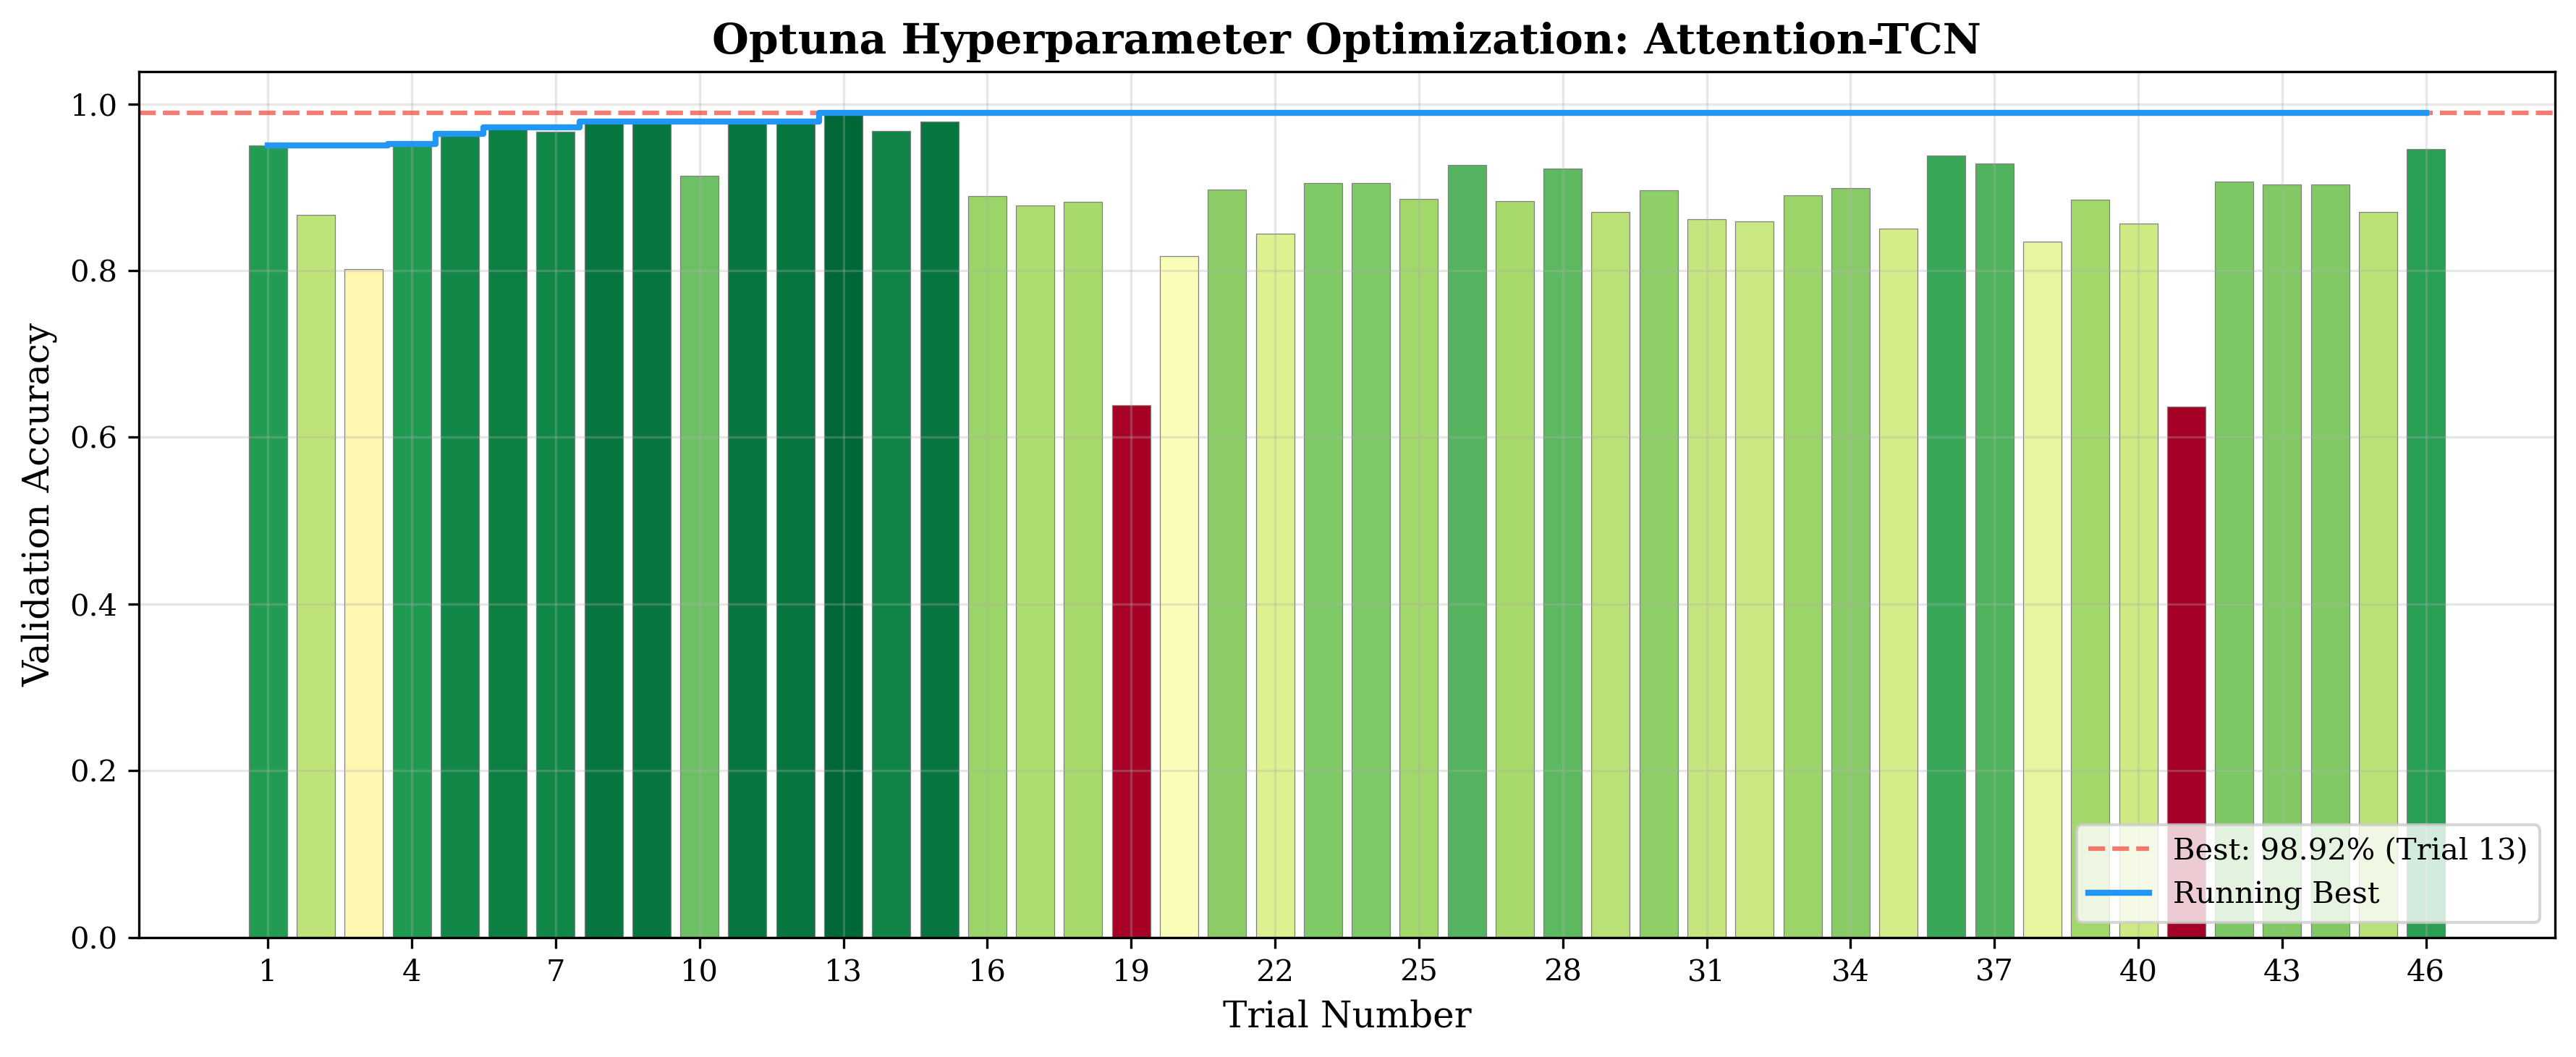
\includegraphics[width=0.95\textwidth]{fig_optuna_trials.png}
\caption{Optuna Hyperparameter Optimization Results}\label{fig_optuna}
\end{figure}

\subsection{Comparative Analysis}
To validate the effectiveness of the Smashifix system, the results were compared against the methods discussed in the Literature Survey. Table \ref{tab_comparative_results} highlights that the Smashifix system now surpasses existing specialized classification models in accuracy while simultaneously providing dynamic biomechanical feedback granularity that other systems lack.

\begin{table}[h]
\caption{Comparative Analysis with State-of-the-Art Methods}\label{tab_comparative_results}
\centering
\setlength{\tabcolsep}{5pt}
\renewcommand{\arraystretch}{1.3}
\begin{tabular}{|l|c|l|l|}
\hline
\textbf{Method} & \textbf{Accuracy} & \textbf{Feedback Type} & \textbf{Scope} \\
\hline
\textbf{Smashifix (Proposed)} & \textbf{98.6\%} & \textbf{Dynamic Biomechanical} & \textbf{Complex Sequence} \\
\hline
Asriani et al. \cite{b18} & 98.6\% & None & Single Stroke \\
\hline
Tukino et al. \cite{b17} & 89.2\% & None & Single Stroke \\
\hline
Bhosale et al. \cite{b32} & 82.0\% & Static Overlay & Static Pose \\
\hline
\end{tabular}
\end{table}

To further validate the approach, Table \ref{tab_cross_sport} compares the proposed system against methods from other sporting domains, demonstrating the generalizability of the dual-pipeline and biomechanical feedback approach.
\clearpage
\begin{table}[h]
\caption{Cross-Sport Comparative Analysis}\label{tab_cross_sport}
\centering
\small
\setlength{\tabcolsep}{4pt}
\renewcommand{\arraystretch}{1.3}
\begin{tabular}{|l|l|c|l|l|}
\hline
\textbf{Method} & \textbf{Sport} & \textbf{Accuracy} & \textbf{Feedback} & \textbf{Input} \\
\hline
Siddiqui et al. \cite{b19} & Cricket & 99.7\% & None & Skeleton \\
\hline
Harini et al. \cite{b33} & Squat Exercise & 91.0\% & Rule-based & Skeleton \\
\hline

\textbf{Smashifix (Proposed)} & \textbf{Badminton} & \textbf{98.6\%} & \textbf{KSI + DTW} & \textbf{Skeleton + Visual} \\
\hline
\end{tabular}
\end{table}

\subsection{System Output Demonstration}
To provide concrete visual evidence of the deployed Smashifix application, this subsection presents representative screenshots captured from the web-based interface during a live analysis session of a Forehand Clear stroke.

Fig.~\ref{fig_analysis_output} displays the Analysis Results panel generated after forensic-mode processing. The system correctly predicts the stroke as a \textit{Forehand Clear} with 77.8\% confidence, identifies the contact frame (Frame~13), and produces a structured Coaching Feedback report. The KSI score of $S = 0.30$ places the user in the ``Foundation Building'' tier, triggering a set of prioritized biomechanical corrections---in this case, a critical $170.0^{\circ}$ deviation in Spine Lateral Lean. Each detected issue is accompanied by a specific fix recommendation and a targeted drill, demonstrating the Natural Language Coach's ability to translate numerical KSI outputs into actionable, skill-appropriate coaching advice.

\begin{figure}[htbp]
\centering
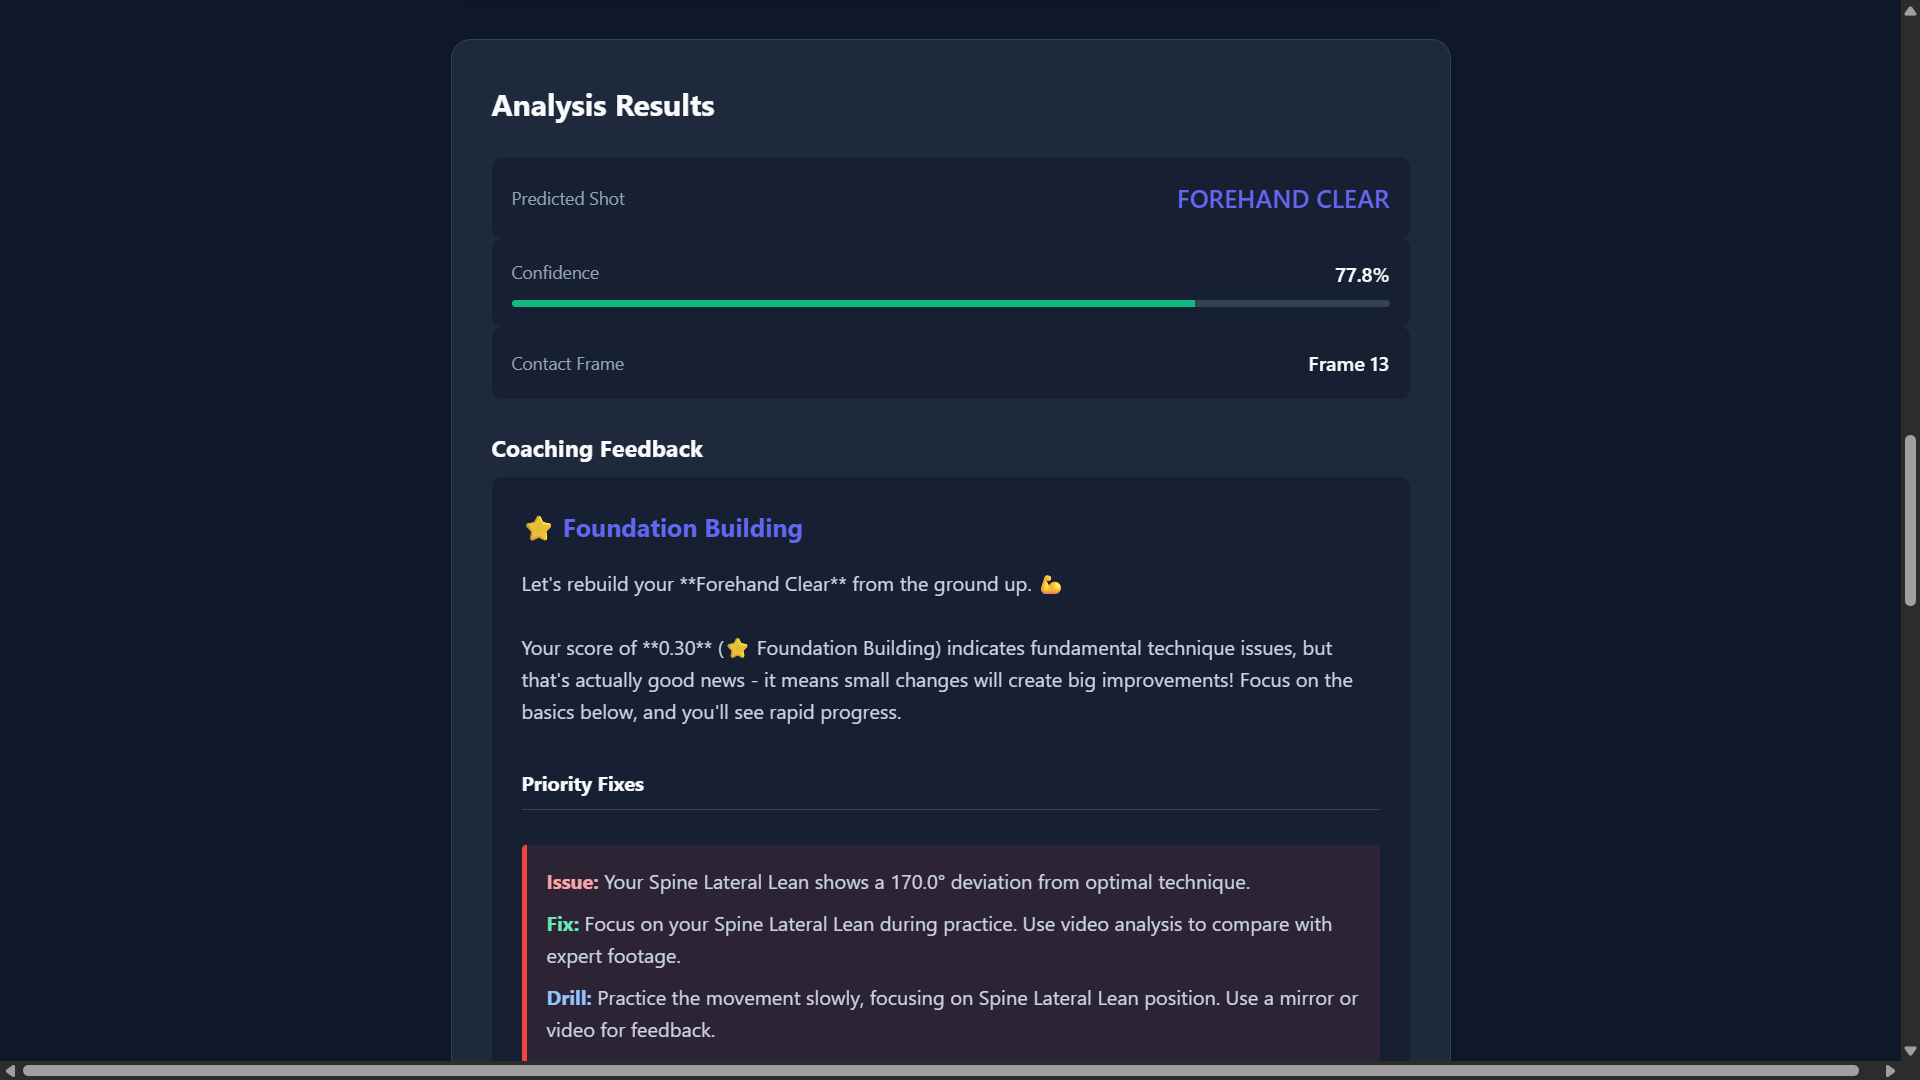
\includegraphics[width=0.85\textwidth]{fig_coaching_output.png}
\caption{Smashifix Analysis Results panel showing stroke classification (Forehand Clear, 77.8\% confidence), contact frame identification, and KSI-driven coaching feedback with prioritized biomechanical corrections and drill recommendations.}\label{fig_analysis_output}
\end{figure}

Fig.~\ref{fig_error_highlight} presents the Error Visualization module, which pinpoints specific biomechanical faults detected during the stroke execution. The interface lists time-stamped error entries (at 00:02.86s, Frame~86) identifying five concurrent deviations: spine lateral lean, spine forward lean, shoulder rotation angle, hip rotation angle, and right knee angle. This granular, frame-level error localization enables players to scrub directly to the problematic moment in the video playback, facilitating targeted review of the exact instant where technique breakdown occurs.

\begin{figure}[htbp]
\centering
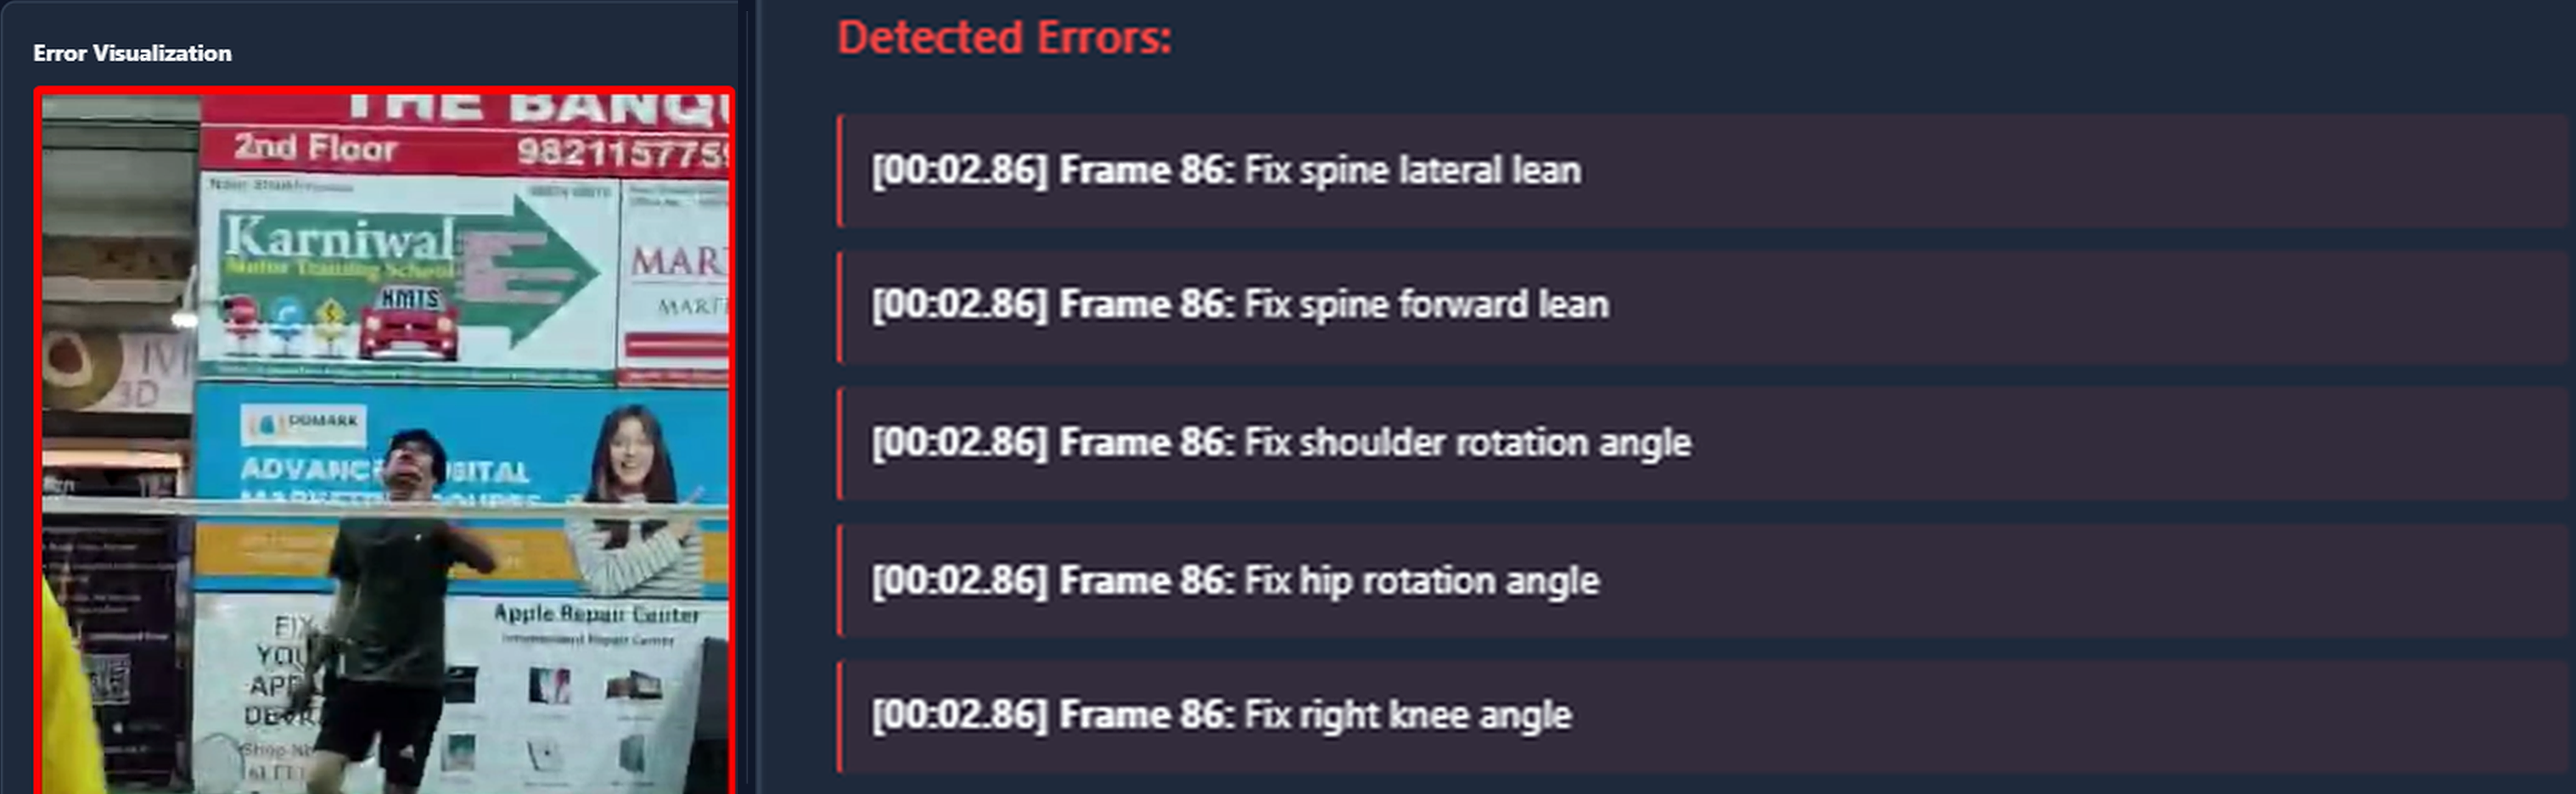
\includegraphics[width=0.85\textwidth]{fig_error_visualization.png}
\caption{Error Visualization panel displaying time-stamped, frame-level biomechanical error detection. Five concurrent deviations are identified at Frame~86, enabling precise temporal localization of technique faults for targeted review.}\label{fig_error_highlight}
\end{figure}

Fig.~\ref{fig_expert_ref} illustrates the Correct Execution (Slow Motion) module, which provides a side-by-side expert reference for the classified stroke. After analysis, the system retrieves and presents a slow-motion video of an elite player performing the same stroke type (in this instance, a Forehand Clear), enabling direct visual comparison between the user's execution and the expert template. This pedagogical feature complements the quantitative KSI feedback by offering an intuitive visual benchmark, allowing players to observe proper biomechanics---including racket arm trajectory, body rotation timing, and follow-through form---at reduced playback speed.

\begin{figure}[htbp]
\centering
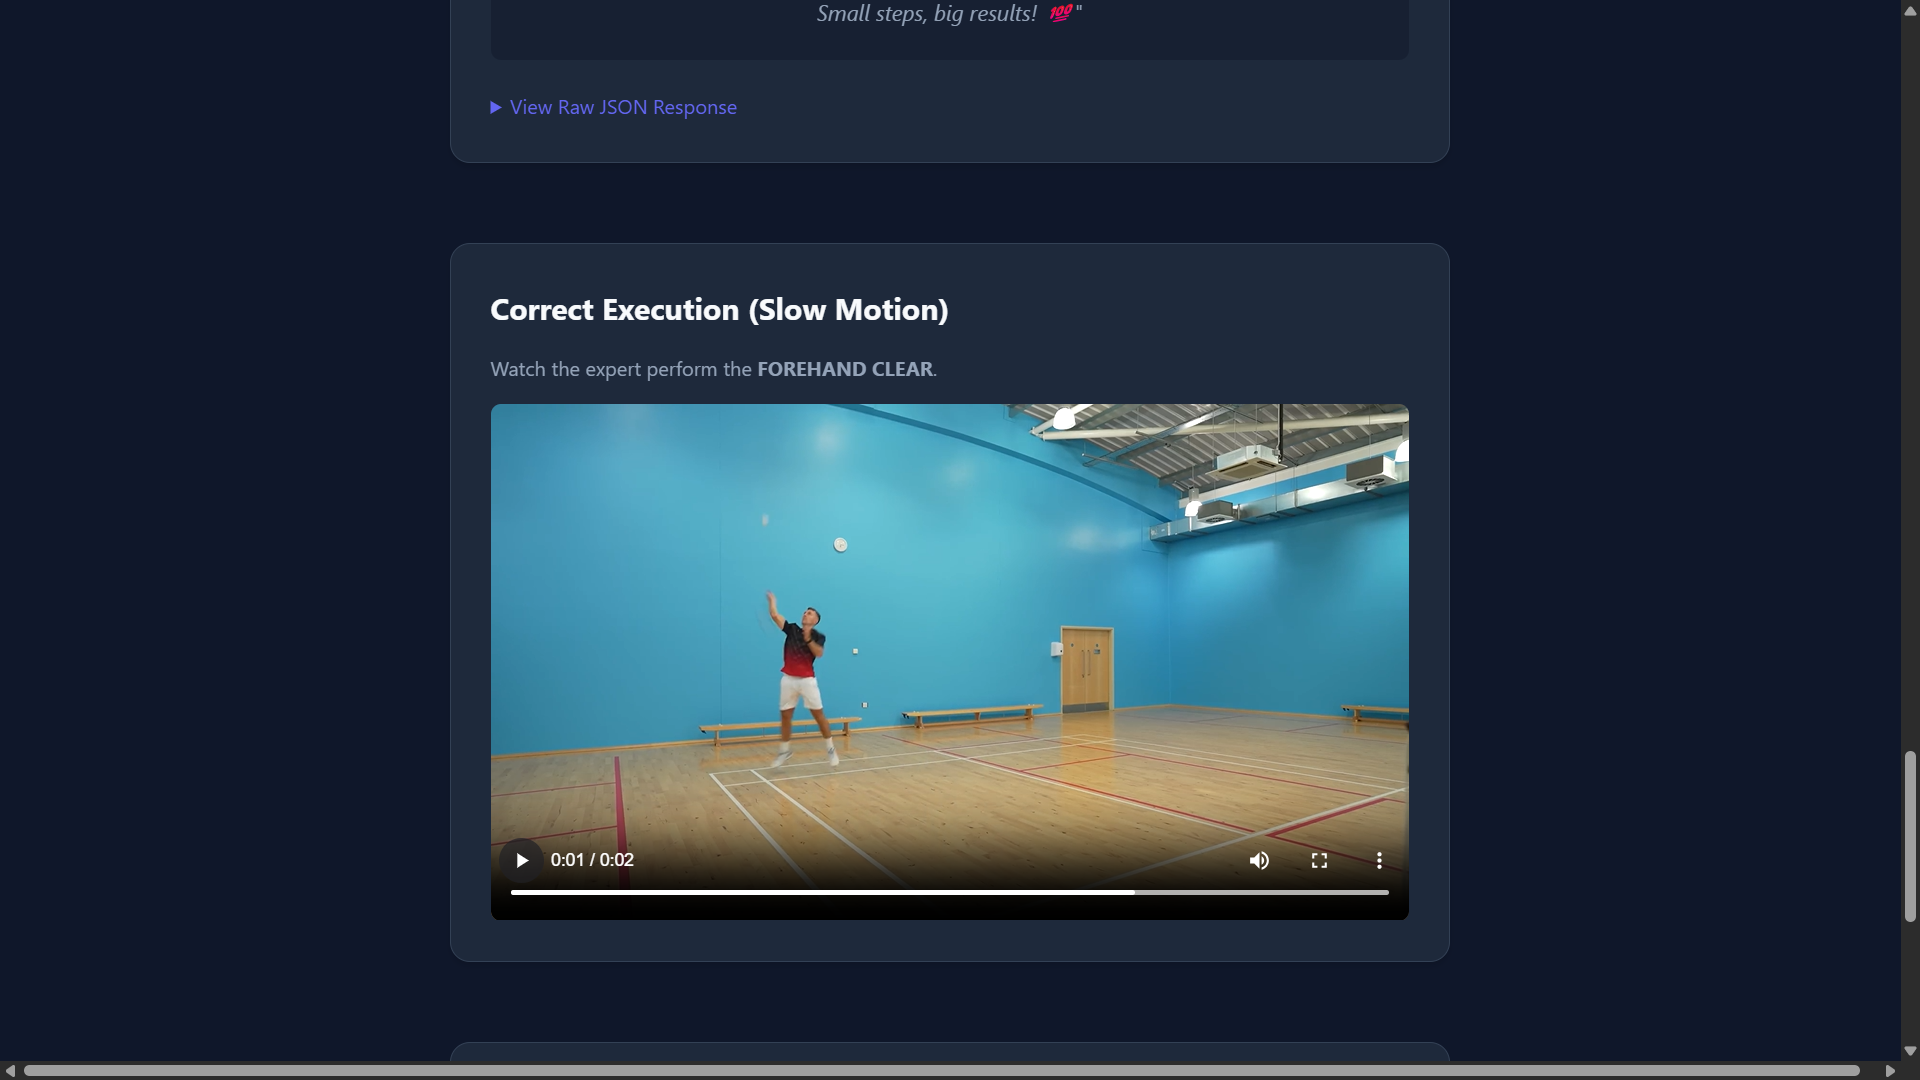
\includegraphics[width=0.85\textwidth]{fig_expert_reference.png}
\caption{Correct Execution (Slow Motion) module displaying expert reference footage for the classified Forehand Clear stroke. The slow-motion playback enables players to visually compare their technique against elite biomechanical form.}\label{fig_expert_ref}
\end{figure}

Collectively, these three output components demonstrate the end-to-end capability of the Smashifix system to transform a single monocular video input into a comprehensive, multi-modal coaching report. Fig.~\ref{fig_analysis_output} shows the quantitative analysis with coaching feedback, Fig.~\ref{fig_error_highlight} illustrates the temporal error localization, and Fig.~\ref{fig_expert_ref} provides the expert visual reference. Together, these components address \textit{what} was performed, \textit{where} errors occurred, \textit{how} to correct them, and \textit{what} correct execution looks like.


\section{Conclusion}\label{sec6}
This paper presented Smashifix, a comprehensive automated coaching system for badminton that bridges the gap between amateur practice and professional-grade biomechanical analysis. The proposed Late-Fusion Dual-Stream Hybrid architecture fuses visual features from a custom Residual-Shuffle Network backbone with 99-dimensional skeletal pose features via an Attention-enhanced Temporal Convolutional Network, delivering high-fidelity forensic analysis with 98.56\% test accuracy and a macro-averaged F1-score of 0.98 across six stroke types. The implementation of a deterministic, configuration-driven spatial cropping strategy successfully eliminated the temporal jitter characteristic of dynamic bounding boxes, ensuring robust and consistent visual stream extraction. The mathematical rigor of the KSI scoring system---employing Sakoe-Chiba constrained DTW, phase-aware attention weighting, 32 hierarchical biomechanical features, and differential kinematics---is seamlessly translated into actionable, skill-appropriate textual drills by an integrated Natural Language Coach. Experimental results demonstrated that Bayesian hyperparameter optimization via Optuna yielded a peak validation accuracy of 98.92\%, confirming the capacity of the architecture when optimally configured. The system was validated against existing state-of-the-art methods and demonstrated superior classification accuracy combined with unmatched feedback granularity, providing sophisticated yet accessible biomechanical analysis that existing systems lack.

Future work offers several promising directions to expand the system's capabilities. Integrating multi-person tracking would extend analysis to doubles matches and crowded environments. A critical area for procedural improvement involves developing a unified, dynamic multi-person tracking mechanism or a self-adjusting bounding box logic that maintains the temporal stability of the current static methodology while actively eliminating the need for manual, per-video configuration overrides. Additionally, deploying quantized models on edge devices like smartphones would democratize access without requiring server-side computation. Incorporating dense surface modeling would also enable deeper analysis of muscle activation and complex torso rotations. Finally, transitioning to data-driven deep metric learning would capture subtler elite motion nuances often missed by hand-engineered features.
\backmatter


\begin{thebibliography}{00}

\bibitem{b1} Bourdon PC et al (2017) Monitoring training load in athletes. Int J Sports Physiol Perform 12:161--170
\bibitem{b2} Cust EE et al (2019) Machine and deep learning for sport-specific movement recognition. J Sports Sci 37(5):568--600
\bibitem{b3} Ribeiro FM et al (2021) Person re-identification in sports: a systematic review. IEEE Access 9
\bibitem{b4} Wang CY et al (2020) Tennis player actions dataset for human pose estimation. IEEE Access 8:12345--12356
\bibitem{b5} Sozykin K et al (2018) Multi-camera human pose estimation and tracking in sports. IEEE/CVF CVPR Workshops
\bibitem{b6} Zhang X et al (2021) Research on badminton teaching technology based on human pose estimation algorithm. Int J Adv Comput Sci Appl 12(5)
\bibitem{b7} Ghosh S et al (2022) Towards automated badminton match analysis: shuttlecock trajectory tracking. Pattern Recognit Lett 158:120--127
\bibitem{b8} Gu C et al (2018) AVA: a video dataset of spatio-temporally localized atomic visual actions. IEEE/CVF CVPR
\bibitem{b9} Dibenedetto G et al (2022) A comprehensive review of deep learning-based human pose estimation. Comput Vis Image Underst 223
\bibitem{b10} Yan S, Xiong Y, Lin D (2018) Spatial temporal graph convolutional networks for skeleton-based action recognition. AAAI
\bibitem{b11} Cao Z, Simon T, Wei SE, Sheikh Y (2017) Realtime multi-person 2D pose estimation using part affinity fields. CVPR
\bibitem{b12} Lugaresi C, Tang J, Nash H et al (2019) MediaPipe: a framework for building perception pipelines. arXiv preprint arXiv:1906.08172
\bibitem{b13} Bazarevsky V, Grishchenko I, Raveendran K et al (2020) BlazePose: on-device real-time body pose tracking. arXiv preprint arXiv:2006.10204
\bibitem{b14} Toshev A, Szegedy C (2014) DeepPose: human pose estimation via deep neural networks. CVPR
\bibitem{b15} G\"uler RA, Neverova N, Kokkinos I (2018) DensePose: dense human pose estimation in the wild. CVPR
\bibitem{b16} Martinez J et al (2017) A simple yet effective baseline for 3d human pose estimation. ICCV
\bibitem{b17} Tukino T et al (2024) Deep learning-based technical classification of badminton pose with CNNs. Int J Artif Intell Res 8(1)
\bibitem{b18} Asriani F et al (2023) A hybrid model of vision transformer and skeleton-based features for badminton. Sensors 23(4)
\bibitem{b19} Siddiqui HUR et al (2023) Enhancing cricket performance analysis with human pose estimation. Procedia Comput Sci 217
\bibitem{b20} Donahue J, Hendricks LA, Guadarrama S et al (2015) Long-term recurrent convolutional networks for visual recognition and description. CVPR
\bibitem{b21} Simonyan K, Zisserman A (2014) Two-stream convolutional networks for action recognition in videos. NeurIPS
\bibitem{b22} Carreira J, Zisserman A (2017) Quo vadis, action recognition? CVPR
\bibitem{b23} Feichtenhofer C et al (2019) SlowFast networks for video recognition. ICCV
\bibitem{b24} Ma N, Zhang X, Zheng HT, Sun J (2018) ShuffleNet V2: practical guidelines for efficient CNN architecture design. ECCV
\bibitem{b25} Samma H, Bin Sama SR (2024) Optimized deep learning vision system for human action recognition from drone images. Multimed Tools Appl 83
\bibitem{b26} Han K et al (2020) GhostNet: more features from cheap operations. CVPR
\bibitem{b27} Pham VT et al (2022) A lightweight graph convolutional network for skeleton-based action recognition. Multimed Tools Appl 81
\bibitem{b28} Yuan J et al (2023) A lightweight graph convolutional network with multi-attention mechanisms for action recognition. Multimed Tools Appl 82
\bibitem{b29} Vaswani A, Shazeer N, Parmar N et al (2017) Attention is all you need. NeurIPS
\bibitem{b30} Yan A et al (2020) Fine-grained abnormal behavior recognition with spatio-temporal attention. IEEE Access 8
\bibitem{b31} Selvaraju RR, Cogswell M, Das A, Vedantam R, Parikh D, Batra D (2017) Grad-CAM: Visual Explanations from Deep Networks via Gradient-Based Localization. ICCV
\bibitem{b32} Bhosale V et al (2021) Yoga pose detection and correction using PoseNet and KNN. Int J Eng Res Technol 10
\bibitem{b33} Harini R et al (2022) Real-time posture correction of squat exercise. Procedia Comput Sci 201
\bibitem{b34} Wang Q (2020) Application of human posture recognition based on the CNN in physical training. J Phys Conf Ser 1533
\bibitem{b35} Stenum J, Ish\o i L (2021) 3D human pose estimation from a single image for biomechanical analysis. J Biomech 120
\bibitem{b36} Nakashima P, Murai Y (2019) Automated baseball pitching analysis using deep learning. ICCV workshops
\bibitem{b37} Liu Y et al (2022) Deep metric learning for motion similarity. IEEE Trans Multimed 24
\bibitem{b38} Doughty H et al (2018) Who's better? Who's best? Pairwise deep ranking for skill determination. CVPR
\bibitem{b39} Pan J et al (2022) Joint-relation-aware network for sports action evaluation. ACM MM

\bibitem{b41} Akiba T, Sano S, Yanase T, Ohta T, Koyama M (2019) Optuna: a next-generation hyperparameter optimization framework. KDD
\bibitem{b42} Sakoe H, Chiba S (1978) Dynamic programming algorithm optimization for spoken word recognition. IEEE TASSP 26(1)
\bibitem{b43} Chang S (2024) Badminton Stroke Video Dataset. Kaggle. \url{https://www.kaggle.com/datasets/shenhuichang/badminton-storke-video}

\end{thebibliography}

\end{document}s